% !TEX program = xelatex
\documentclass[11pt,a4paper]{article}

\usepackage[margin=2.2cm]{geometry}
\usepackage{fontspec}
\usepackage{xeCJK}
\setCJKmainfont{Microsoft YaHei}[BoldFont=Microsoft YaHei Bold,AutoFakeBold=true]
\setCJKsansfont{Microsoft YaHei}
\setCJKmonofont{Microsoft YaHei}
\setmainfont{Times New Roman}
\setsansfont{Arial}
\setmonofont{Consolas}

\usepackage{amsmath,amssymb}
\usepackage{booktabs}
\usepackage{tabularx}
\usepackage{graphicx}
\usepackage{float}
\usepackage{caption}
\usepackage{subcaption}
\usepackage{hyperref}
\usepackage{xcolor}
\usepackage{enumitem}
\usepackage{listings}
\usepackage{multirow}
\usepackage{array}
\usepackage{siunitx}
\usepackage{longtable}
\usepackage{url}

\hypersetup{colorlinks=true,linkcolor=black!70,urlcolor=blue!50!black,citecolor=black!70}
\captionsetup{font=small,labelfont=bf}
\graphicspath{{../outputs/figures/}{../outputs/3d/figures/}}
\newcolumntype{Y}{>{\raggedright\arraybackslash}X}
\newcommand{\dT}{\Delta T}
\newcommand{\code}[1]{\texttt{#1}}
\lstset{basicstyle=\ttfamily\small,breaklines=true,frame=single,backgroundcolor=\color{gray!8},columns=fullflexible}

\title{\bfseries 基于图神经网络的芯片封装二维/三维稳态热场代理模型\\[0.4em]
\large 统一技术说明文档（chip-thermal-gnn）}
\author{项目可复现基线报告：二维流程 + 三维四面体 FEM 扩展}
\date{2026 年 9 月 2 日}

\begin{document}
\maketitle
\begin{center}
\small 本报告以 \code{docs/report.tex} 的 XeLaTeX 排版体系为基础重建；所有标注为“实测”的数值均可追溯到 \code{outputs/} 下的 JSON、CSV、图像或测试记录。
\end{center}
\tableofcontents
\newpage

% =========================================================
\section{项目概述与结论摘要}
% =========================================================

\subsection{任务定义}
本项目构建从封装结构、材料、热源和边界条件到节点温升场的图神经网络代理模型。完整闭环为
\begin{center}
\fbox{\parbox{0.91\textwidth}{\centering
参数化封装与工况 $\rightarrow$ P1 FEM 求解 $\rightarrow$ 网格转 PyG 图 $\rightarrow$ GNN 训练 $\rightarrow$ 场/峰值/OOD/成本评估 $\rightarrow$ 云图解释。}}
\end{center}

二维版本使用三角形 FEM 和 $x$ 方向热点；三维版本保留二维文件与数据契约，新增真实 \textbf{四面体 FEM}、Die 中的 $x$--$z$ 平面矩形热点和三维 PyG 图。温度标签均来自开源 \code{scikit-fem} 的实际数值求解，而非解析近似或虚构数据 \cite{skfem}。

\subsection{当前可复现结论}
\begin{itemize}[leftmargin=1.5em]
  \item 三维 GraphSAGE 是当前可信主基线：测试集 MAE \textbf{0.0835 K}、峰值温升误差 \textbf{0.1206 K}、加权 OOD MAE \textbf{0.1866 K}；三维紧凑 MeshGraphNet 暂未超过它。
  \item 三维四面体实现已经过真实 \code{scikit-fem} 测试和制造解（MMS）网格收敛验证：\textbf{6 passed}，观测收敛阶为 1.677 与 1.830。
  \item 差对流 \code{ood\_poor\_cooling} 是最明显的外推短板；三维 GraphSAGE 的该组 MAE 为 0.5283 K，应优先改善边界表示和训练覆盖，而非盲目增加消息传递深度。
  \item 二维与三维均使用 300/30/30 的固定种子数据划分；三维具有更丰富的横向扩散信息，但四面体图的边数与 FEM 成本显著增加。
\end{itemize}

\subsection{范围与非目标}
本报告的目标是建立可复现的研究基线，而不是签核级热仿真。当前不包含温度相关材料参数、辐射、显式接触热阻、各向异性、封装翘曲、几何公差、瞬态热容或实验测温校准。所有“优于”结论仅在所述数据、网格、硬件和超参数下成立。

% =========================================================
\section{物理模型与有限元理论}
% =========================================================

\subsection{分层几何与材料}
二维结构为 $20\,\mathrm{mm}\times12\,\mathrm{mm}$ 的封装截面；三维结构在此基础上增加 $16\,\mathrm{mm}$ 深度。两者均由下而上包含 Substrate、Cu、TIM 与 Die 四层。

\begin{figure}[H]
  \centering
  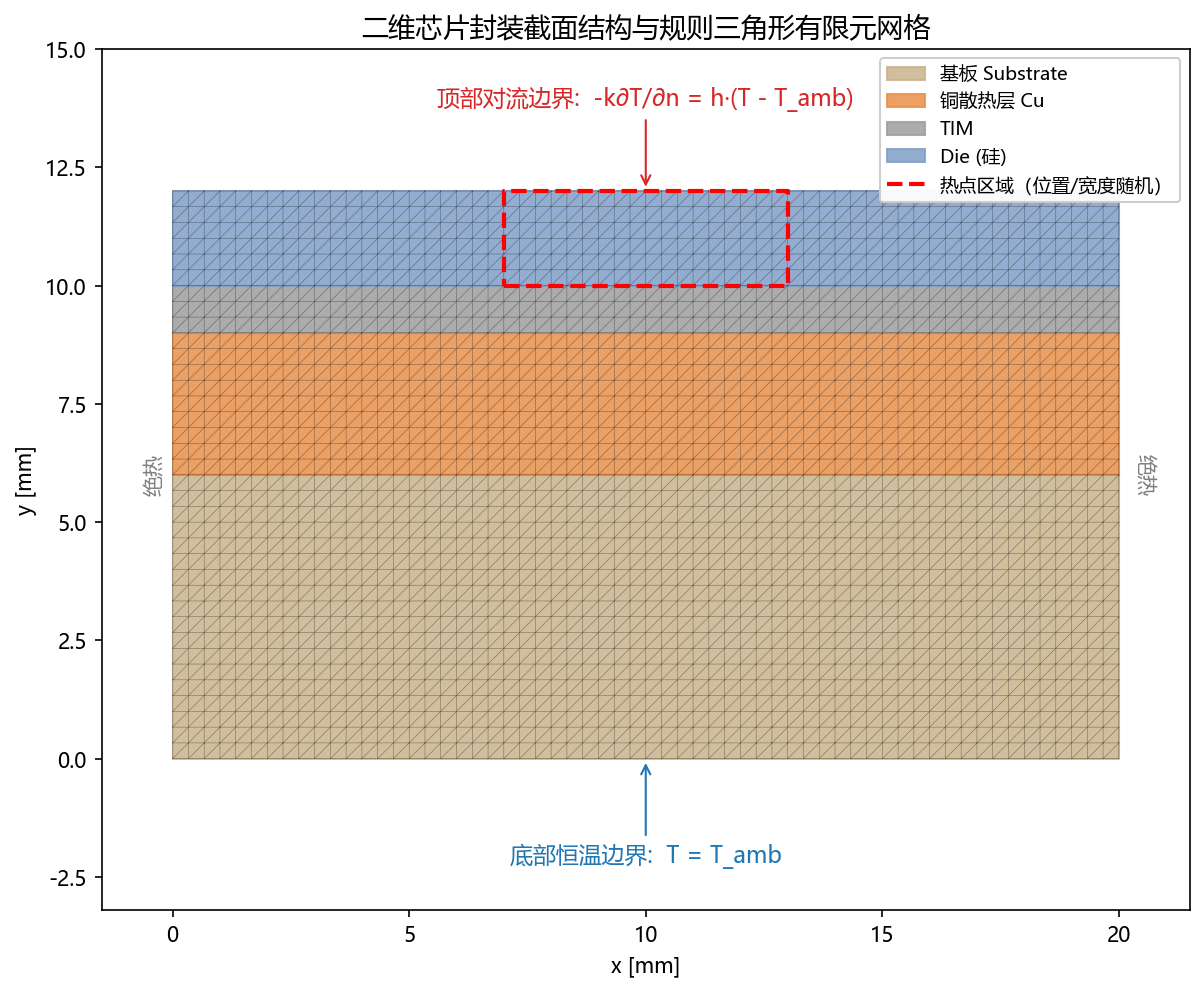
\includegraphics[width=0.92\textwidth]{package_structure_mesh.png}
  \caption{二维封装截面、分层材料、三角形网格与热点示意。三维版本沿 $z$ 方向扩展为体域，并把热点定义为 $x$--$z$ 平面矩形。}
  \label{fig:structure}
\end{figure}

\begin{table}[H]
\centering
\caption{层级、厚度与材料采样范围}
\label{tab:layers}
\begin{tabular}{llcc}
\toprule
层级 & 材料示意 & 厚度 & 导热系数 $k$ [W/(m$\cdot$K)] \\
\midrule
Substrate & 有机/陶瓷类 & 6 mm & $15\sim60$ \\
Cu & 铜散热层 & 3 mm & $360\sim400$ \\
TIM & 导热界面材料 & 1 mm & $1\sim8$（OOD: $0.2\sim0.9$） \\
Die & 硅芯片 & 2 mm & $130\sim155$ \\
\bottomrule
\end{tabular}
\end{table}

\subsection{控制方程和边界条件}
在 $d\in\{2,3\}$ 维域 $\Omega$ 内，求解稳态热传导方程
\begin{equation}
-\nabla\cdot\left(k(\mathbf{x})\nabla T(\mathbf{x})\right)=q(\mathbf{x}),\qquad \mathbf{x}\in\Omega,
\label{eq:steady}
\end{equation}
其中 $k$ 是分材料导热系数，$q$ 是体热源密度。边界条件为
\begin{align}
T &= T_{amb}, && \text{on }\Gamma_{bottom}, \label{eq:dirichlet}\\
-k\nabla T\cdot\mathbf{n} &= h_{top}(T-T_{amb}), && \text{on }\Gamma_{top}, \label{eq:robin}\\
-k\nabla T\cdot\mathbf{n} &=0, && \text{on }\Gamma_{side}. \label{eq:neumann}
\end{align}

这里底部为理想散热地，顶面为 Robin 对流，二维侧边或三维剩余侧面为绝热。由于当前模型线性且所有边界均以 $T_{amb}$ 为参考，学习目标采用
\begin{equation}
\dT(\mathbf{x})=T(\mathbf{x})-T_{amb}.
\end{equation}
改变 $T_{amb}$ 仅平移绝对温度而不改变 $\dT$；该变量仍作为已知条件保留，以适配未来温度相关物性的非线性扩展。

\subsection{弱式与 P1 单元}
令 $V_0=\{v\in H^1(\Omega):v|_{\Gamma_{bottom}}=0\}$。弱式为：求满足 Dirichlet 条件的 $T$，使任意 $v\in V_0$ 满足
\begin{equation}
\int_\Omega k\nabla T\cdot\nabla v\,d\Omega+
\int_{\Gamma_{top}}h_{top}Tv\,d\Gamma=
\int_\Omega qv\,d\Omega+
\int_{\Gamma_{top}}h_{top}T_{amb}v\,d\Gamma.
\label{eq:weak}
\end{equation}

二维采用 3 节点线性三角元，三维采用 4 节点线性四面体。单元近似与局部装配为
\begin{equation}
T_h|_{e}=\sum_{i=1}^{n_e}N_iT_i,\qquad
K^{(e)}_{ij}=\int_{\Omega_e}k\nabla N_i\cdot\nabla N_j\,d\Omega,\qquad
f_i^{(e)}=\int_{\Omega_e}qN_i\,d\Omega,
\end{equation}
其中 $n_e=3$（二维）或 4（三维）。三维顶面三角形 $s$ 的 Robin 局部矩阵为
\begin{equation}
K^{(s)}_{R}=\frac{h_{top}A_s}{12}
\begin{bmatrix}2&1&1\\1&2&1\\1&1&2\end{bmatrix},
\end{equation}
右端增加 $h_{top}T_{amb}A_s/3$。实现直接使用 scikit-fem 的稀疏形式组装、约束消元和求解 \cite{skfem}。

\subsection{热源参数化}
二维 Die 内热点由中心 $x_c$ 与宽度 $w_x$ 定义。三维 Die 内热点是 $x$--$z$ 矩形，沿 Die 厚度方向 $y$ 延展：
\begin{equation}
q(x,y,z)=\begin{cases}
q_{hot},& y>y_{TIM},\ x\in[x_c-w_x/2,x_c+w_x/2],\ z\in[z_c-w_z/2,z_c+w_z/2],\\
q_{base},& y>y_{TIM}\ \text{且不在热点内},\\
0,& \text{其他层}.
\end{cases}
\label{eq:hotspot}
\end{equation}

\begin{table}[H]
\centering
\caption{工况采样与分布外测试范围}
\label{tab:ranges}
\begin{tabular}{lcc}
\toprule
量 & 分布内范围 & OOD 范围（仅测试集部分样本） \\
\midrule
$q_{base}$ [W/m$^3$] & $1\times10^5\sim5\times10^5$ & -- \\
$q_{hot}$ [W/m$^3$] & $5\times10^6\sim3\times10^7$ & $3.5\times10^7\sim6\times10^7$ \\
$h_{top}$ [W/(m$^2\cdot$K)] & $500\sim15000$ & $100\sim400$ \\
$T_{amb}$ [$^\circ$C] & $20\sim45$ & 同分布内 \\
\bottomrule
\end{tabular}
\end{table}

% =========================================================
\section{数据集与 PyG 图构建}
% =========================================================

\subsection{数据拆分与可重复性}
二维和完整三维数据集均使用随机种子 2024，训练/验证/测试划分均为 300/30/30。测试集由 20 个分布内样本与 10 个 OOD 样本组成，覆盖高功率、低 TIM 导热和弱对流工况。所有样本保存工况元数据和 FEM 求解时间；温升均值/标准差仅从训练拆分统计，避免测试标签泄漏。

\begin{table}[H]
\centering
\caption{二维与三维 FEM--图数据规格}
\label{tab:graph-spec}
\begin{tabular}{lcc}
\toprule
属性 & 二维流程 & 三维流程 \\
\midrule
有限元单元 & P1 三角形 & P1 四面体 \\
规则网格 & $61\times37$ & $13\times13\times11$ \\
节点数 & 2,257 & 1,859 \\
单元数 & 4,320 三角形 & 8,640 四面体 \\
有向边数 & 13,152 & 22,532 \\
节点特征维度 & 21 & 24 \\
边特征维度 & 4 & 5 \\
标签 & 节点温升 $\dT$ & 节点温升 $\dT$ \\
\bottomrule
\end{tabular}
\end{table}

三维节点数略少于二维，但四面体的 6 条顶点对导致边数增加约 71\%。处理时对每个三角形或四面体的无向顶点对去重，再保留两个方向写入 \code{edge\_index}；图中不含自环。

\subsection{节点与边特征}
节点特征由可观测局部量和广播到所有节点的全局工况量构成：归一化坐标、4 类材料 one-hot、局部热源、环境温度、局部对流系数、顶/底边界标志、热点几何、材料导热率与热阻式变量 $1/k_{TIM}$、$1/h_{top}$。二维坐标为 $(x/W,y/H)$，三维额外加入 $z/D$；因此三维热点全局量额外包含 $z_c,w_z$。

边特征为归一化相对位移、边长和端点材料导热率调和平均
\begin{equation}
k_{ij}=\frac{2k_ik_j}{k_i+k_j}.
\end{equation}
三维边特征新增 $\Delta z/D$。全局工况广播不是温度标签泄漏：它只提供部署时同样可知的设计参数。这样做的原因是稳态导热为全局耦合的椭圆型问题，有限消息传递步数不足以可靠地把远端热源或边界信息传过整个图。

处理后的样本使用 \code{torch\_geometric.data.Data} 保存，含 \code{x}、\code{edge\_index}、\code{edge\_attr}、\code{y} 与 \code{pos}。PyTorch Geometric 为不规则图、图批处理与相关图卷积提供支持 \cite{pyg}。

% =========================================================
\section{网络架构与训练方法}
% =========================================================

\begin{figure}[H]
  \centering
  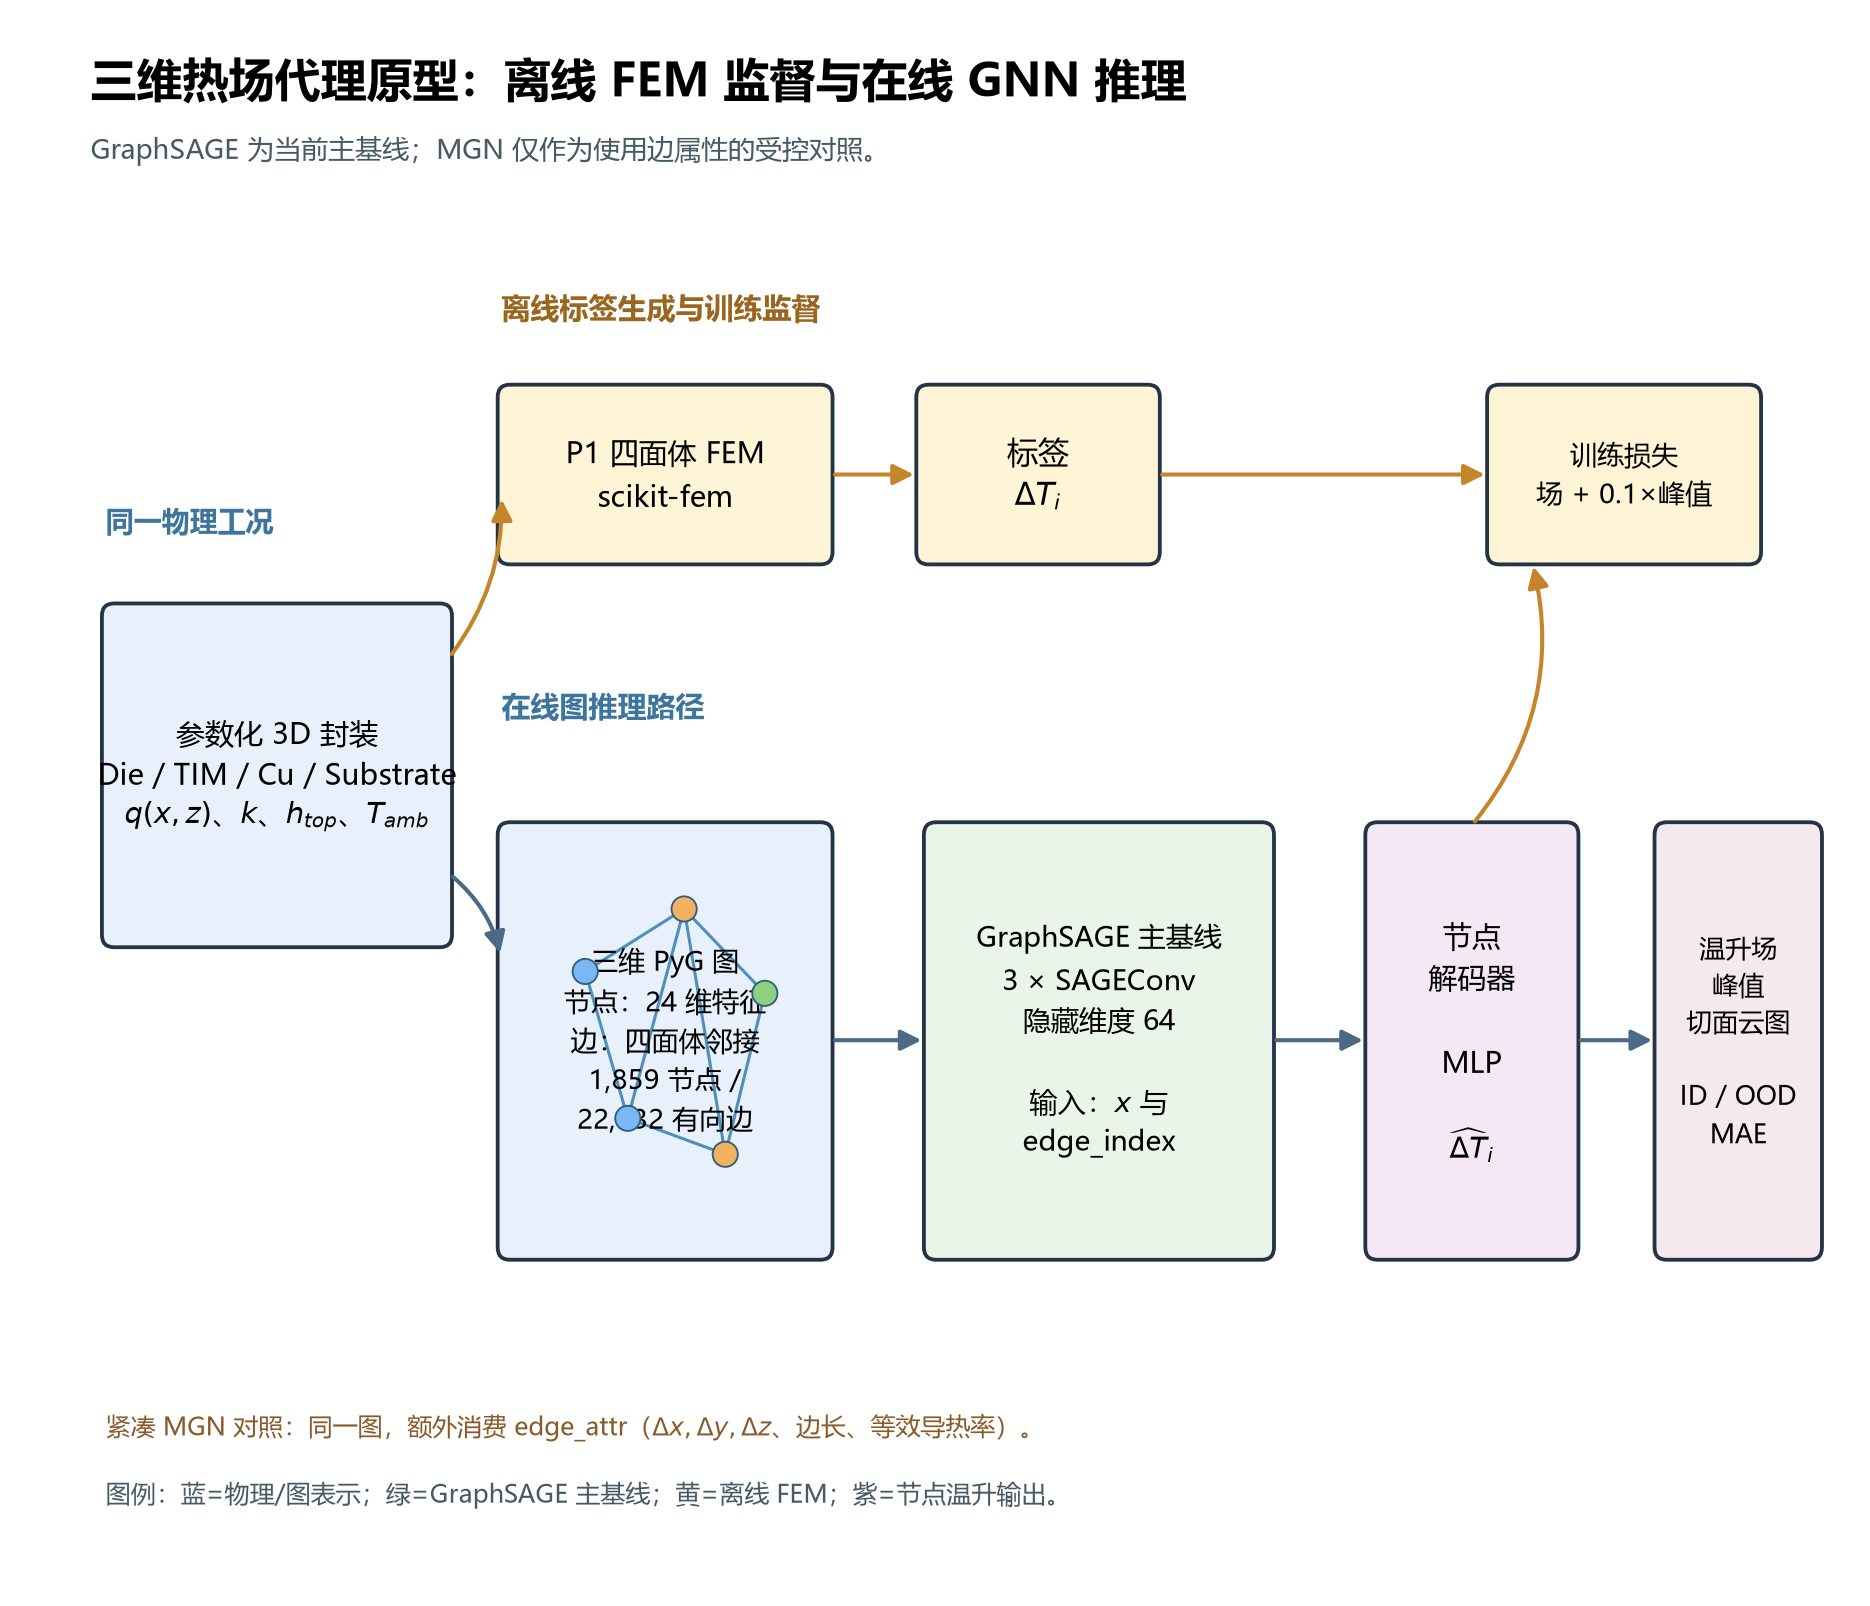
\includegraphics[width=0.96\textwidth]{thermal_gnn_prototype_compact.png}
  \caption{三维芯片封装热场 GNN 原型，置于网络架构章节以对应后续 GraphSAGE 与 MGN 说明。离线支路通过 \code{scikit-fem} 的 P1 四面体 FEM 产生监督标签；在线支路将 24 维节点特征和四面体邻接送入 3 层、隐藏维度 64 的 GraphSAGE，逐节点输出温升场。边属性在数据中保留给紧凑 MGN 对照，当前 GraphSAGE 主基线仅使用 \code{edge\_index} 与节点特征。}
  \label{fig:method-pipeline}
\end{figure}

\subsection{GraphSAGE 基线}
GraphSAGE 是归纳图学习方法 \cite{graphsage}。其均值聚合的简化表达为
\begin{equation}
\mathbf{h}_{v}^{(\ell+1)}=\sigma\left(W^{(\ell)}\left[\mathbf{h}_{v}^{(\ell)}\Vert
\operatorname{mean}_{u\in\mathcal{N}(v)}\mathbf{h}_{u}^{(\ell)}\right]\right).
\label{eq:sage}
\end{equation}
本项目的 GraphSAGE 直接回归节点标准化温升，不消费 \code{edge\_attr}。它是必要的低复杂度基线，用于判断复杂边消息网络是否真正带来收益。

\subsection{MeshGraphNet 风格 Encode--Process--Decode}
MeshGraphNets 将网格表示为节点和边图，以编码、残差消息传递和解码器学习仿真映射 \cite{mgn}。本项目仅借鉴其架构思想，模型在本地独立实现、从零训练，未复用任何外部权重或源码。第 $\ell$ 步消息传递可写为
\begin{align}
\mathbf{e}_{ij}^{(\ell+1)}&=\mathbf{e}_{ij}^{(\ell)}+\phi_e([\mathbf{h}_i^{(\ell)},\mathbf{h}_j^{(\ell)},\mathbf{e}_{ij}^{(\ell)}]),\\
\mathbf{m}_i^{(\ell+1)}&=\sum_{j:(j,i)\in E}\mathbf{e}_{ji}^{(\ell+1)},\\
\mathbf{h}_i^{(\ell+1)}&=\mathbf{h}_i^{(\ell)}+\phi_v([\mathbf{h}_i^{(\ell)},\mathbf{m}_i^{(\ell+1)}]),\\
\widehat{\dT}_i&=\psi(\mathbf{h}_i^{(L)}).
\end{align}
节点/边 MLP 使用 LayerNorm、dropout 与残差连接。MGN 消费边的几何与等效导热特征，因此在三维大边数图中会显著提高状态与聚合成本。

\begin{table}[H]
\centering
\caption{模型与训练配置}
\label{tab:model-config}
\begin{tabular}{lcccc}
\toprule
配置 & 2D GraphSAGE & 2D MGN & 3D GraphSAGE & 3D 紧凑 MGN \\
\midrule
层/消息步 & 4 层 & 8 步 & 3 层 & 2 步 \\
隐藏维度 & 128 & 128 & 64 & 64 \\
参数量 & 104,321 & 979,329 & 19,713 & 73,153 \\
batch size & 8 & 8 & 4 & 8 \\
训练轮上限 & 500 & 500 & 120 & 12 \\
CPU 线程约束 & 历史配置 & 历史配置 & 4 & 4 \\
\bottomrule
\end{tabular}
\end{table}

三维 MGN 特意先采用 2--4 步、64 或 96 维的紧凑搜索方向，而没有直接照搬二维的 8 步、128 维。原因是 3D 图的每条有向边都有边隐状态和 MLP 计算，过大的初始配置会使成本迅速膨胀。

\subsection{损失函数、优化和早停}
令 $z$ 为使用训练拆分均值/标准差标准化后的温升。主损失采用逐样本相对能量形式：
\begin{equation}
\mathcal{L}_{field}=\frac{1}{B}\sum_{b=1}^{B}
\frac{\sum_{i\in b}(\hat{z}_i-z_i)^2}
{\sum_{i\in b}(z_i-\bar{z}_b)^2+10^{-4}}.
\label{eq:field-loss}
\end{equation}
真实峰值节点 $i_b^*=\arg\max_{i\in b}z_i$ 处的辅助损失为
\begin{equation}
\mathcal{L}=\mathcal{L}_{field}+0.1\cdot\frac{1}{B}\sum_b(\hat{z}_{i_b^*}-z_{i_b^*})^2.
\label{eq:loss}
\end{equation}
该设计避免高温升样本支配训练，并强化工程上关心的热点峰值。优化器为 Adam（初始学习率 $10^{-3}$）、\code{ReduceLROnPlateau}、梯度裁剪 1.0、固定种子 2024 和验证集早停。

\begin{figure}[H]
  \centering
  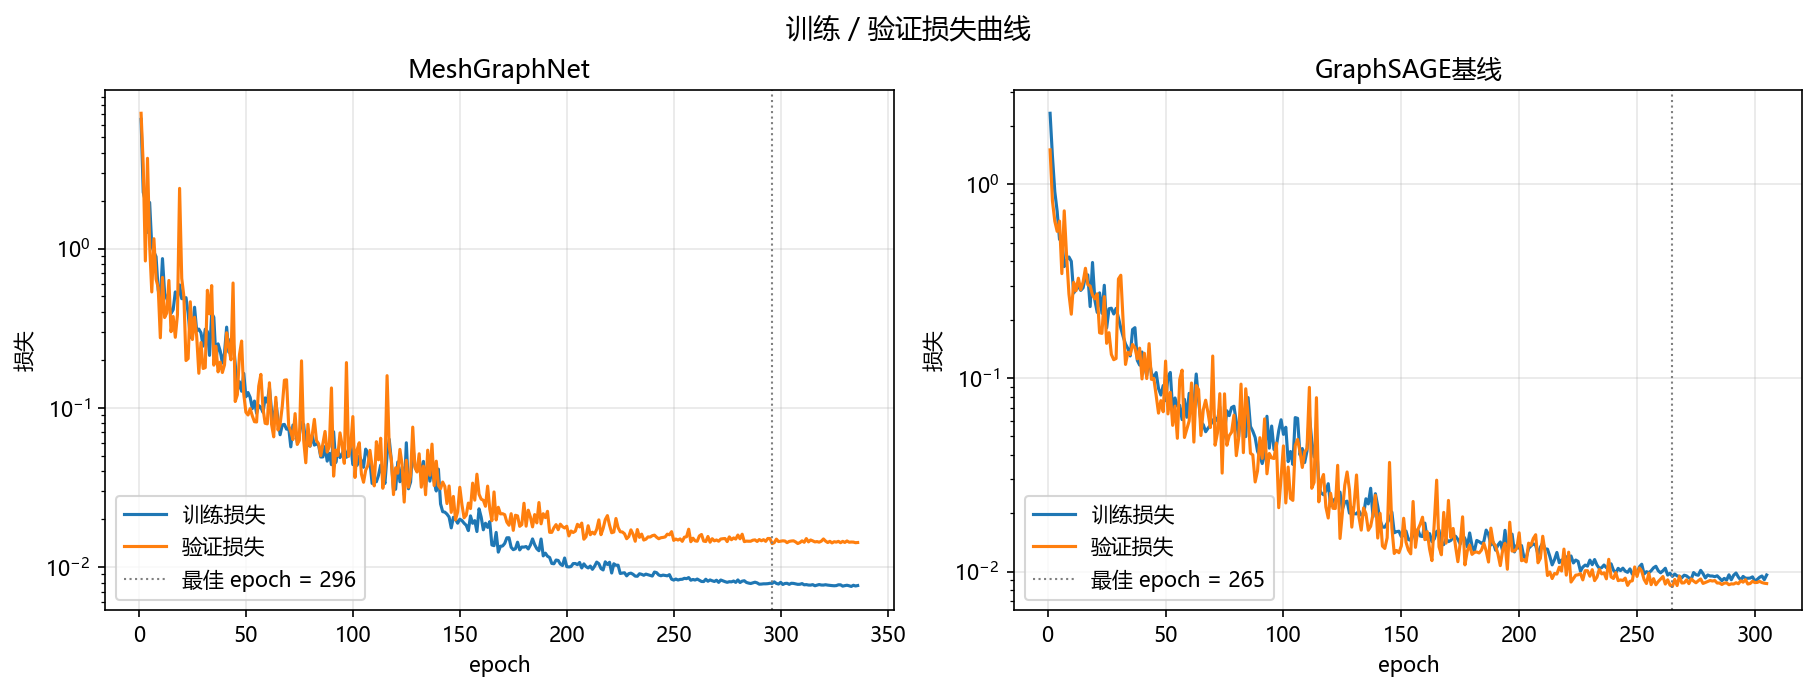
\includegraphics[width=0.97\textwidth]{loss_curves.png}
  \caption{二维历史训练的 MeshGraphNet 与 GraphSAGE 训练/验证损失曲线。该图用于展示二维流程收敛，不与三维紧凑 MGN 的训练轮数混比。}
  \label{fig:loss}
\end{figure}

% =========================================================
\section{验证与测试方案}
% =========================================================

\subsection{分层测试原则}
测试被分为物理一致性、数据契约、网络可训练性和数值收敛四层。物理直觉测试可发现热源、边界和分层实现错误；数据契约测试可发现网格转图错误；网络前后向测试验证可训练性；MMS 独立验证离散随网格加密的数值行为。

\begin{table}[H]
\centering
\caption{二维与三维测试覆盖及证据状态}
\label{tab:test-plan}
\begin{tabularx}{\textwidth}{lYY}
\toprule
层级 & 测试内容 & 证据状态 \\
\midrule
2D FEM & 温度有限、底部恒温、最高温在 Die、热源增大时峰值增大、材料层编号 & \code{tests/test\_fem\_solver.py} 已定义；本次统一报告未重新运行 \\
2D 图数据 & 三角形转双向去重边、无自环、21/4 维特征、处理文件形状 & \code{tests/test\_graph\_dataset.py} 已定义；本次未重新运行 \\
2D 网络 & MGN 前向/反向梯度、GraphSAGE 与 GCN 前向形状 & \code{tests/test\_models.py} 已定义；本次未重新运行 \\
3D FEM/图 & 四面体连通、边界、$x$--$z$ 热点、双向边、24/5 维特征 & 已实际运行并通过 \\
3D MMS & 网格加密误差单调下降、收敛阶阈值 & 已实际运行并通过 \\
\bottomrule
\end{tabularx}
\end{table}

二维测试代码和二维训练评估产物都保留在仓库中，但没有同一日期的二维 \code{pytest} 终端日志，因此本报告不将其误写为“本轮通过”。如需重新确认，命令为 \code{python -m pytest tests -q}；根据项目约定，应在运行前取得授权。

\subsection{三维真实后端测试}
实际执行的命令为
\begin{lstlisting}
.\.venv-3d\Scripts\python.exe -m pytest \
  tests/test_fem_solver_3d.py tests/test_graph_dataset_3d.py \
  tests/test_mms_3d.py -q
\end{lstlisting}
结果为 \textbf{6 passed}，另有两条 PyTorch \code{torch.jit.script} 弃用警告，不影响 FEM 或图数据计算。

\subsection{制造解（MMS）收敛验证}
仅依靠“温度升高”“热点在 Die”不足以验证四面体离散。为此，在单位立方体选择解析解
\begin{equation}
T^*(x,y,z)=\sin(\pi x)\sin(\pi y)\sin(\pi z),\qquad q=3\pi^2T^*,
\label{eq:mms}
\end{equation}
并在全部边界施加与解析解一致的零 Dirichlet 条件。MMS 的验证理念参考 MOOSE 热传导验证教程 \cite{moose}，但本仓库的网格、装配、求解和测试均独立执行。

\begin{table}[H]
\centering
\caption{3D P1 四面体 MMS 网格收敛实测结果}
\label{tab:mms}
\begin{tabular}{rrrrr}
\toprule
每轴节点数 & 节点数 & 四面体数 & 节点 RMSE & 最大绝对误差 \\
\midrule
5 & 125 & 384 & $2.4351\times10^{-2}$ & $9.5072\times10^{-2}$ \\
9 & 729 & 3,072 & $7.6178\times10^{-3}$ & $2.5201\times10^{-2}$ \\
13 & 2,197 & 10,368 & $3.6276\times10^{-3}$ & $1.1324\times10^{-2}$ \\
\bottomrule
\end{tabular}
\end{table}

相邻网格观测收敛阶为 \textbf{1.677} 与 \textbf{1.830}，误差随加密单调下降。这证明 P1 四面体实现对光滑解析解具有预期的收敛趋势，但不等同于真实封装实验验证。

\subsection{学习代理的评估指标}
对测试节点或每个样本的温升真值 $\dT$ 与预测 $\widehat{\dT}$，报告
\begin{align}
\mathrm{MAE}&=\frac{1}{N}\sum_i|\widehat{\dT}_i-\dT_i|,\\
\mathrm{RelL2}&=\frac{\|\widehat{\dT}-\dT\|_2}{\|\dT\|_2},\\
E_{peak}&=|\max_i\widehat{\dT}_i-\max_i\dT_i|,
\end{align}
以及 $R^2$、分工况 OOD MAE、单样本/批处理推理时间、FEM 时间与进程 RSS。不同硬件、线程数、batch 和模型大小的速度不得直接混合比较。

% =========================================================
\section{二维流程的已有结果}
% =========================================================

\subsection{训练摘要}
二维产物位于 \code{outputs/metrics/}。GraphSAGE 最佳验证 epoch 为 265，共训练 305 epoch，训练时间 231.57 s；MGN 最佳 epoch 为 296，共训练 336 epoch，训练时间 3,394.16 s。二维 GraphSAGE 当前保存评估的精度为
\begin{table}[H]
\centering
\caption{二维 GraphSAGE 当前保存评估摘要（CPU 记录）}
\label{tab:2d-baseline}
\begin{tabular}{lr}
\toprule
指标 & 数值 \\
\midrule
参数量 & 104,321 \\
整体 MAE & 0.1035 K \\
相对 $L_2$ & 0.2231 \\
$R^2$ & 0.9270 \\
平均峰值温升绝对误差 & 0.3431 K \\
ID / 高功率 / 差 TIM / 差对流 MAE & 0.0308 / 0.1166 / 0.2156 / 0.4589 K \\
平均 FEM 时间 & 8.50 ms \\
单样本 / 批处理推理 & 54.94 / 56.01 ms/样本 \\
评估进程 RSS & 520.09 MiB \\
\bottomrule
\end{tabular}
\end{table}

仓库旧版二维 PDF 中的 MGN 推理时间来自 RTX 3060 历史运行，不能与表~\ref{tab:2d-baseline} 的 CPU 记录或三维 CPU 记录直接比较。二维结果表明在小网格上 FEM 本身很快，代理模型的价值主要体现在批量工况扫描、反复优化或更大规模网格场景。

\begin{figure}[H]
  \centering
  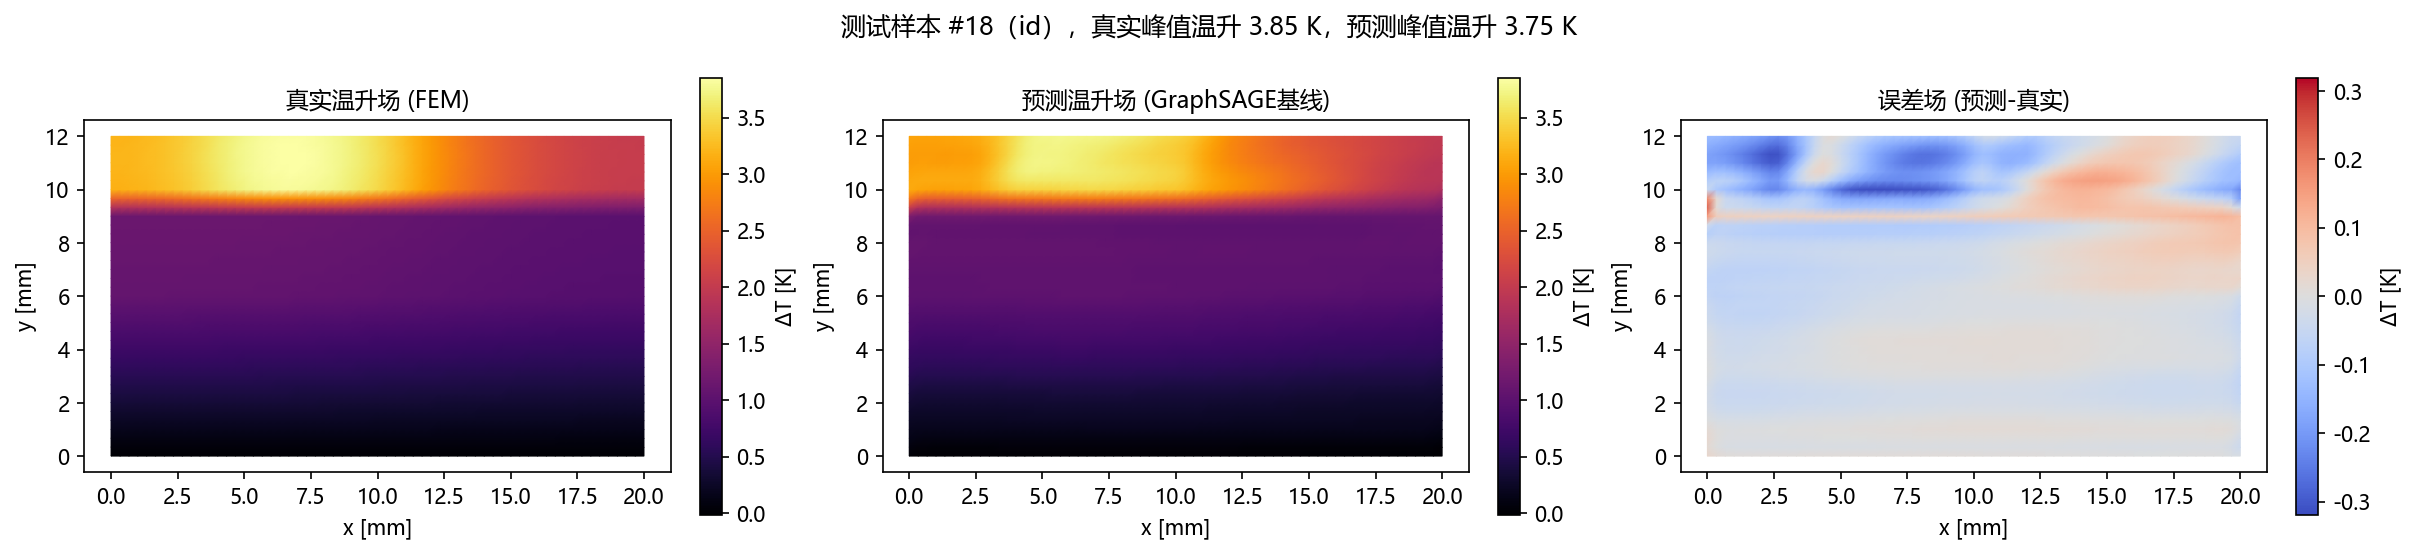
\includegraphics[width=0.96\textwidth]{field_triptych_baseline_sample18.png}
  \caption{二维 GraphSAGE 代表样本：FEM 温升、预测温升与误差场三联图。}
  \label{fig:2d-field}
\end{figure}

\begin{figure}[H]
  \centering
  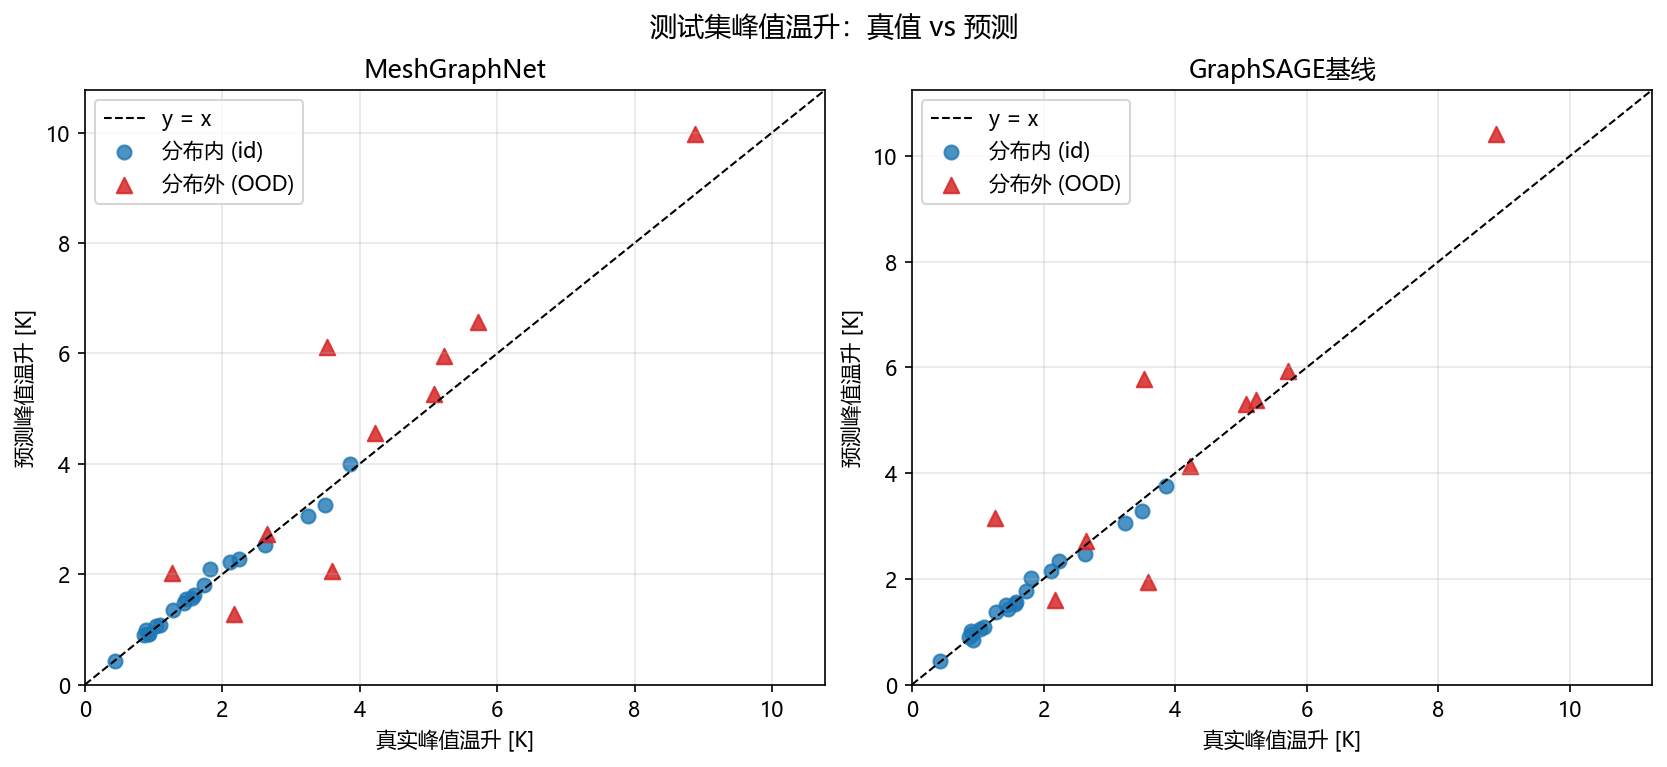
\includegraphics[width=0.88\textwidth]{peak_scatter.png}
  \caption{二维测试集峰值温升真值--预测散点图；图中 OOD 样本用于观察外推误差。}
  \label{fig:2d-peak}
\end{figure}

% =========================================================
\section{三维流程、结果与云图}
% =========================================================

\subsection{三维数据生成与资源规模}
三维完整数据集保存在 \code{data/raw\_3d\_full/} 与 \code{data/processed\_3d\_full/}。300/30/30 个样本的原始 FEM 生成耗时 39.41 s；全部样本平均单次 FEM 求解时间为 92.61 ms，测试评估平均为 112.25 ms。小规模烟雾数据集的温升范围为 0.2987--2.1923 K，单图张量约 0.972 MiB；完整处理集的训练图文件约 189.4 MiB。

\subsection{GraphSAGE 可信基线与紧凑 MGN 探针}
\begin{table}[H]
\centering
\caption{三维模型实测结果（CPU）}
\label{tab:3d-results}
\resizebox{\textwidth}{!}{%
\begin{tabular}{lrrrrrrrr}
\toprule
模型 & 最佳/总 epoch & 参数量 & 训练时间 [s] & MAE [K] & RelL2 & $R^2$ & 峰值误差 [K] & OOD MAE [K] \\
\midrule
GraphSAGE & 69 / 94 & 19,713 & 439.29 & \textbf{0.0835} & \textbf{0.4945} & \textbf{0.6509} & \textbf{0.1206} & \textbf{0.1866} \\
紧凑 MGN & 11 / 12 & 73,153 & 343.80 & 0.1433 & 0.7079 & 0.2846 & 0.1529 & 0.3060 \\
\bottomrule
\end{tabular}}
\end{table}

\begin{table}[H]
\centering
\caption{三维计算成本与 OOD 分拆}
\label{tab:3d-cost-ood}
\begin{tabular}{lcc}
\toprule
指标 & 3D GraphSAGE & 3D 紧凑 MGN \\
\midrule
训练 RSS 峰值 & 597.64 MiB & 887.57 MiB \\
评估 RSS & 600.84 MiB & 1,434.16 MiB \\
单样本 / 批处理推理 & 7.43 / 6.43 ms & 19.13 / 20.98 ms \\
平均 FEM 时间 & 112.25 ms & 112.25 ms \\
ID MAE & 0.0319 K & 0.0620 K \\
高功率 OOD MAE & 0.0489 K & 0.1875 K \\
差 TIM OOD MAE & 0.0283 K & 0.0652 K \\
差对流 OOD MAE & 0.5283 K & 0.7048 K \\
\bottomrule
\end{tabular}
\end{table}

在当前相同数据划分下，GraphSAGE 在精度、OOD、推理时间和内存上都优于紧凑 MGN。因此 GraphSAGE 是冻结的三维主基线；MGN 的 12 epoch 结果只说明小配置尚未学习充分，不能据此推断其理论上无效。

\begin{figure}[H]
  \centering
  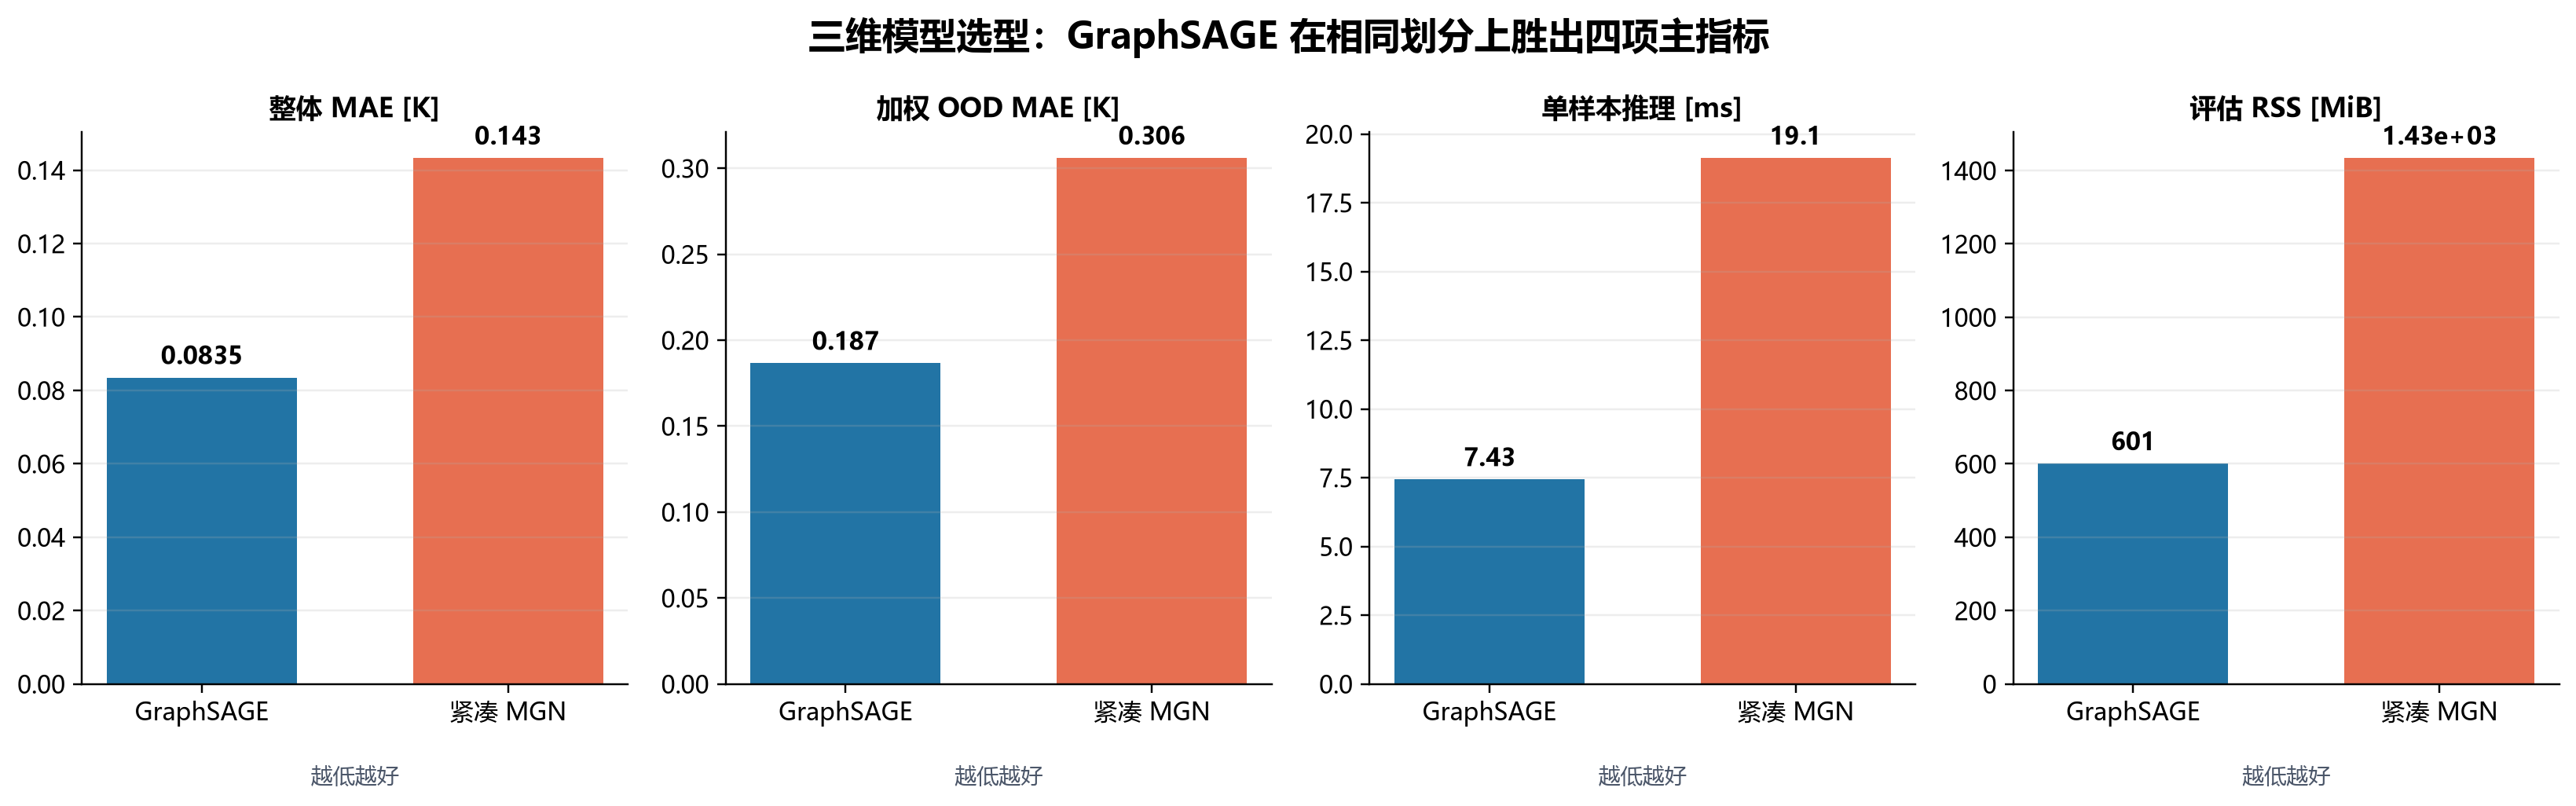
\includegraphics[width=0.98\textwidth]{model_selection_graphsage_3d.png}
  \caption{三维模型选型图。对整体 MAE、按 OOD 样本数加权的 OOD MAE、单样本推理时间和评估 RSS 四项用于当前决策的指标，GraphSAGE 均优于本轮紧凑 MGN；因此主推 GraphSAGE 是实测选择，而非架构偏好。}
  \label{fig:model-selection}
\end{figure}

\begin{figure}[H]
  \centering
  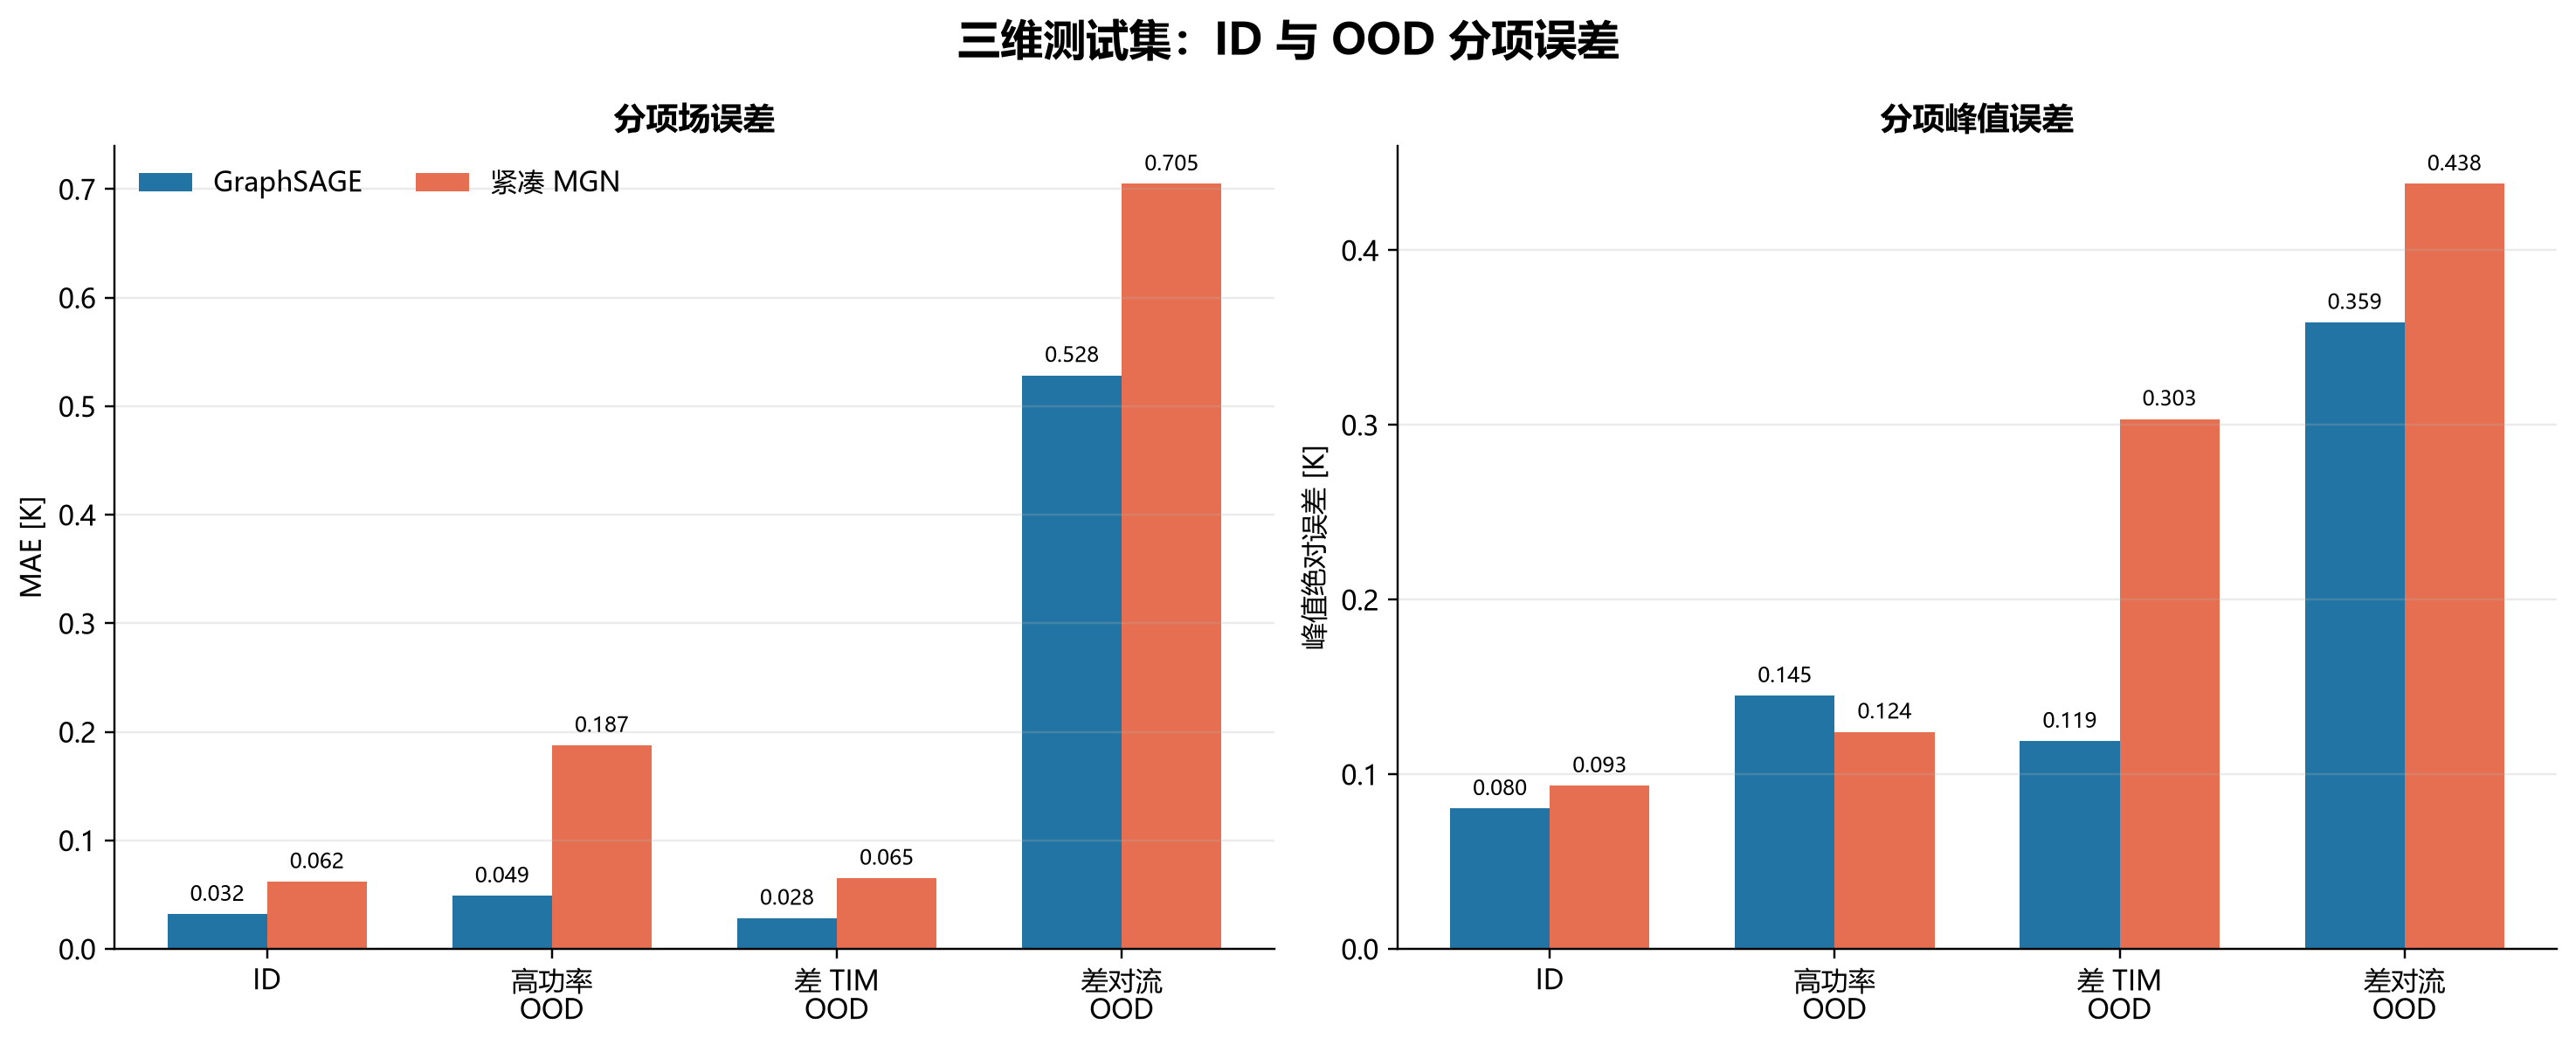
\includegraphics[width=0.98\textwidth]{ood_error_breakdown_3d.png}
  \caption{ID 与 OOD 分项误差。差对流是两个模型共同的最大难例；高功率下 MGN 的峰值误差略小，但其场 MAE、其他 OOD 组别和总体成本均不占优。图用于定位后续物理覆盖，而非把单一平均数当作充分结论。}
  \label{fig:ood-breakdown}
\end{figure}

\subsection{三维切面云图}
每张三维图按列展示 FEM、GNN 预测和预测减 FEM 的误差；按行展示 Die 中心 $x$--$z$ 热点平面、中心 $y$--$z$ 平面和中心 $x$--$y$ 平面。

\begin{figure}[H]
  \centering
  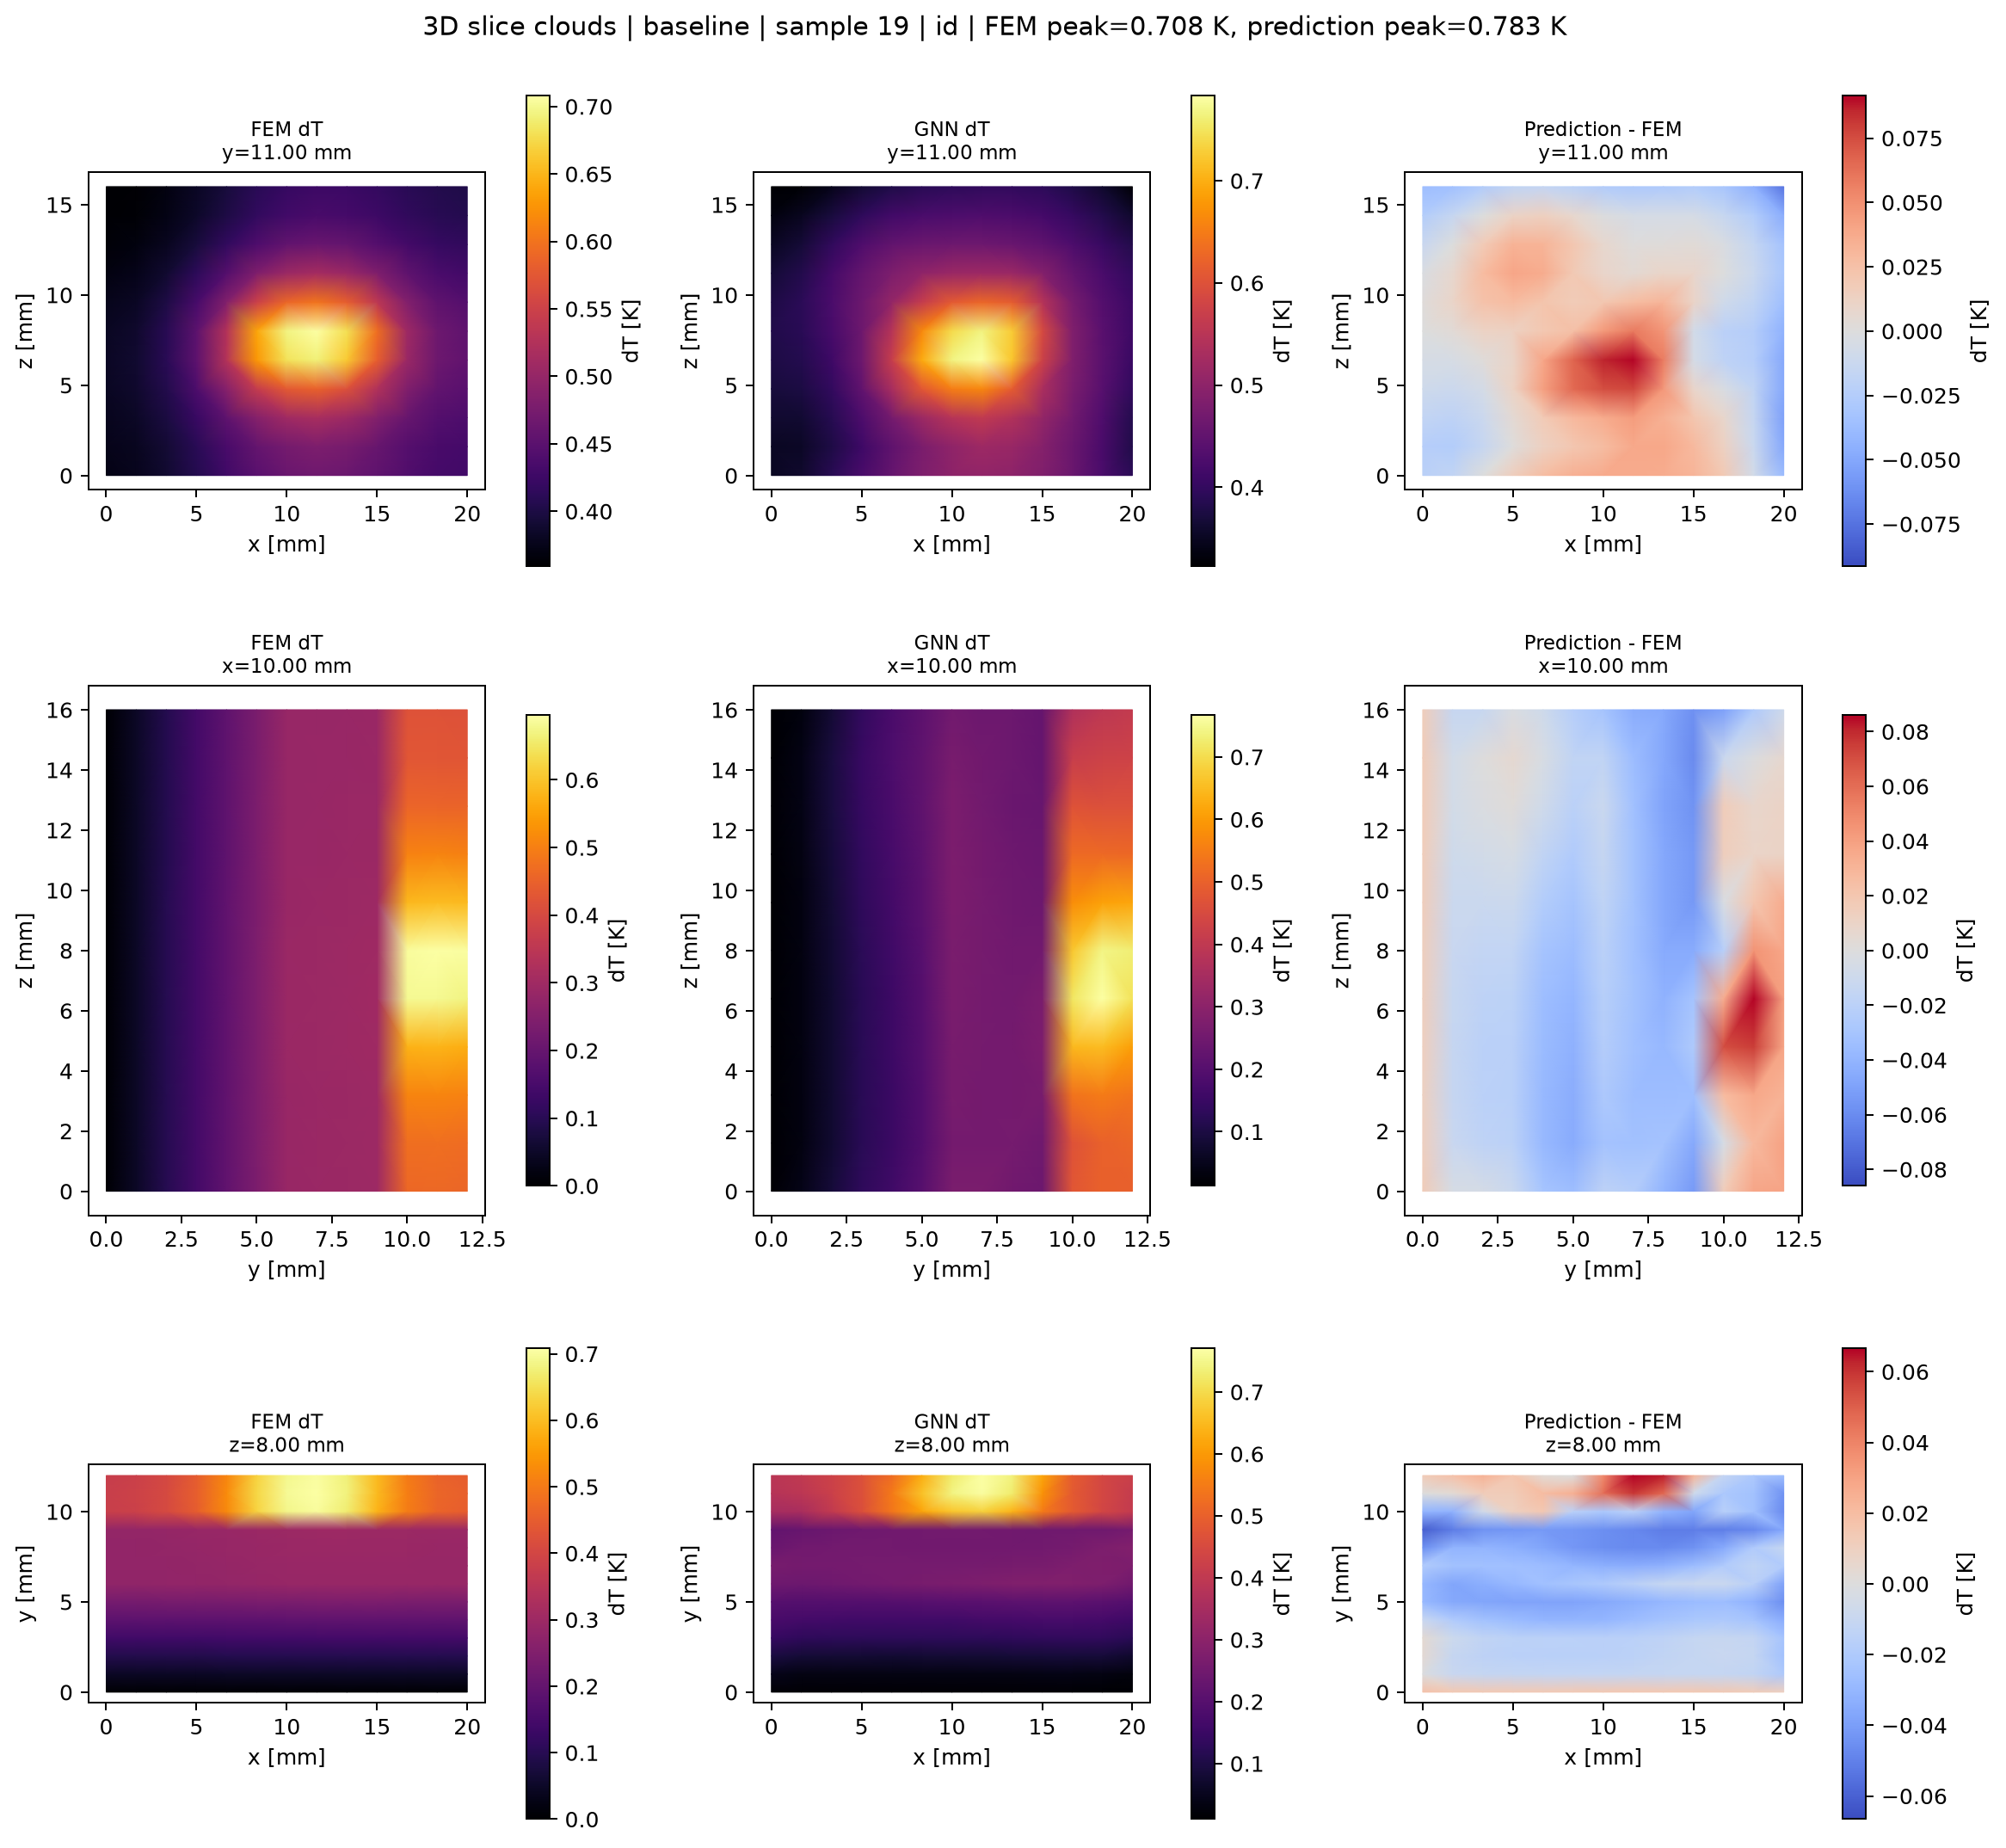
\includegraphics[width=0.98\textwidth]{slice_clouds_baseline_sample19_id.png}
  \caption{三维 GraphSAGE：中位 ID 样本 \#19。FEM 峰值 0.708 K，预测峰值 0.783 K。热点位置和厚度方向热扩散得到重建，误差主要集中在热点周围和材料界面。}
  \label{fig:3d-id}
\end{figure}

\begin{figure}[H]
  \centering
  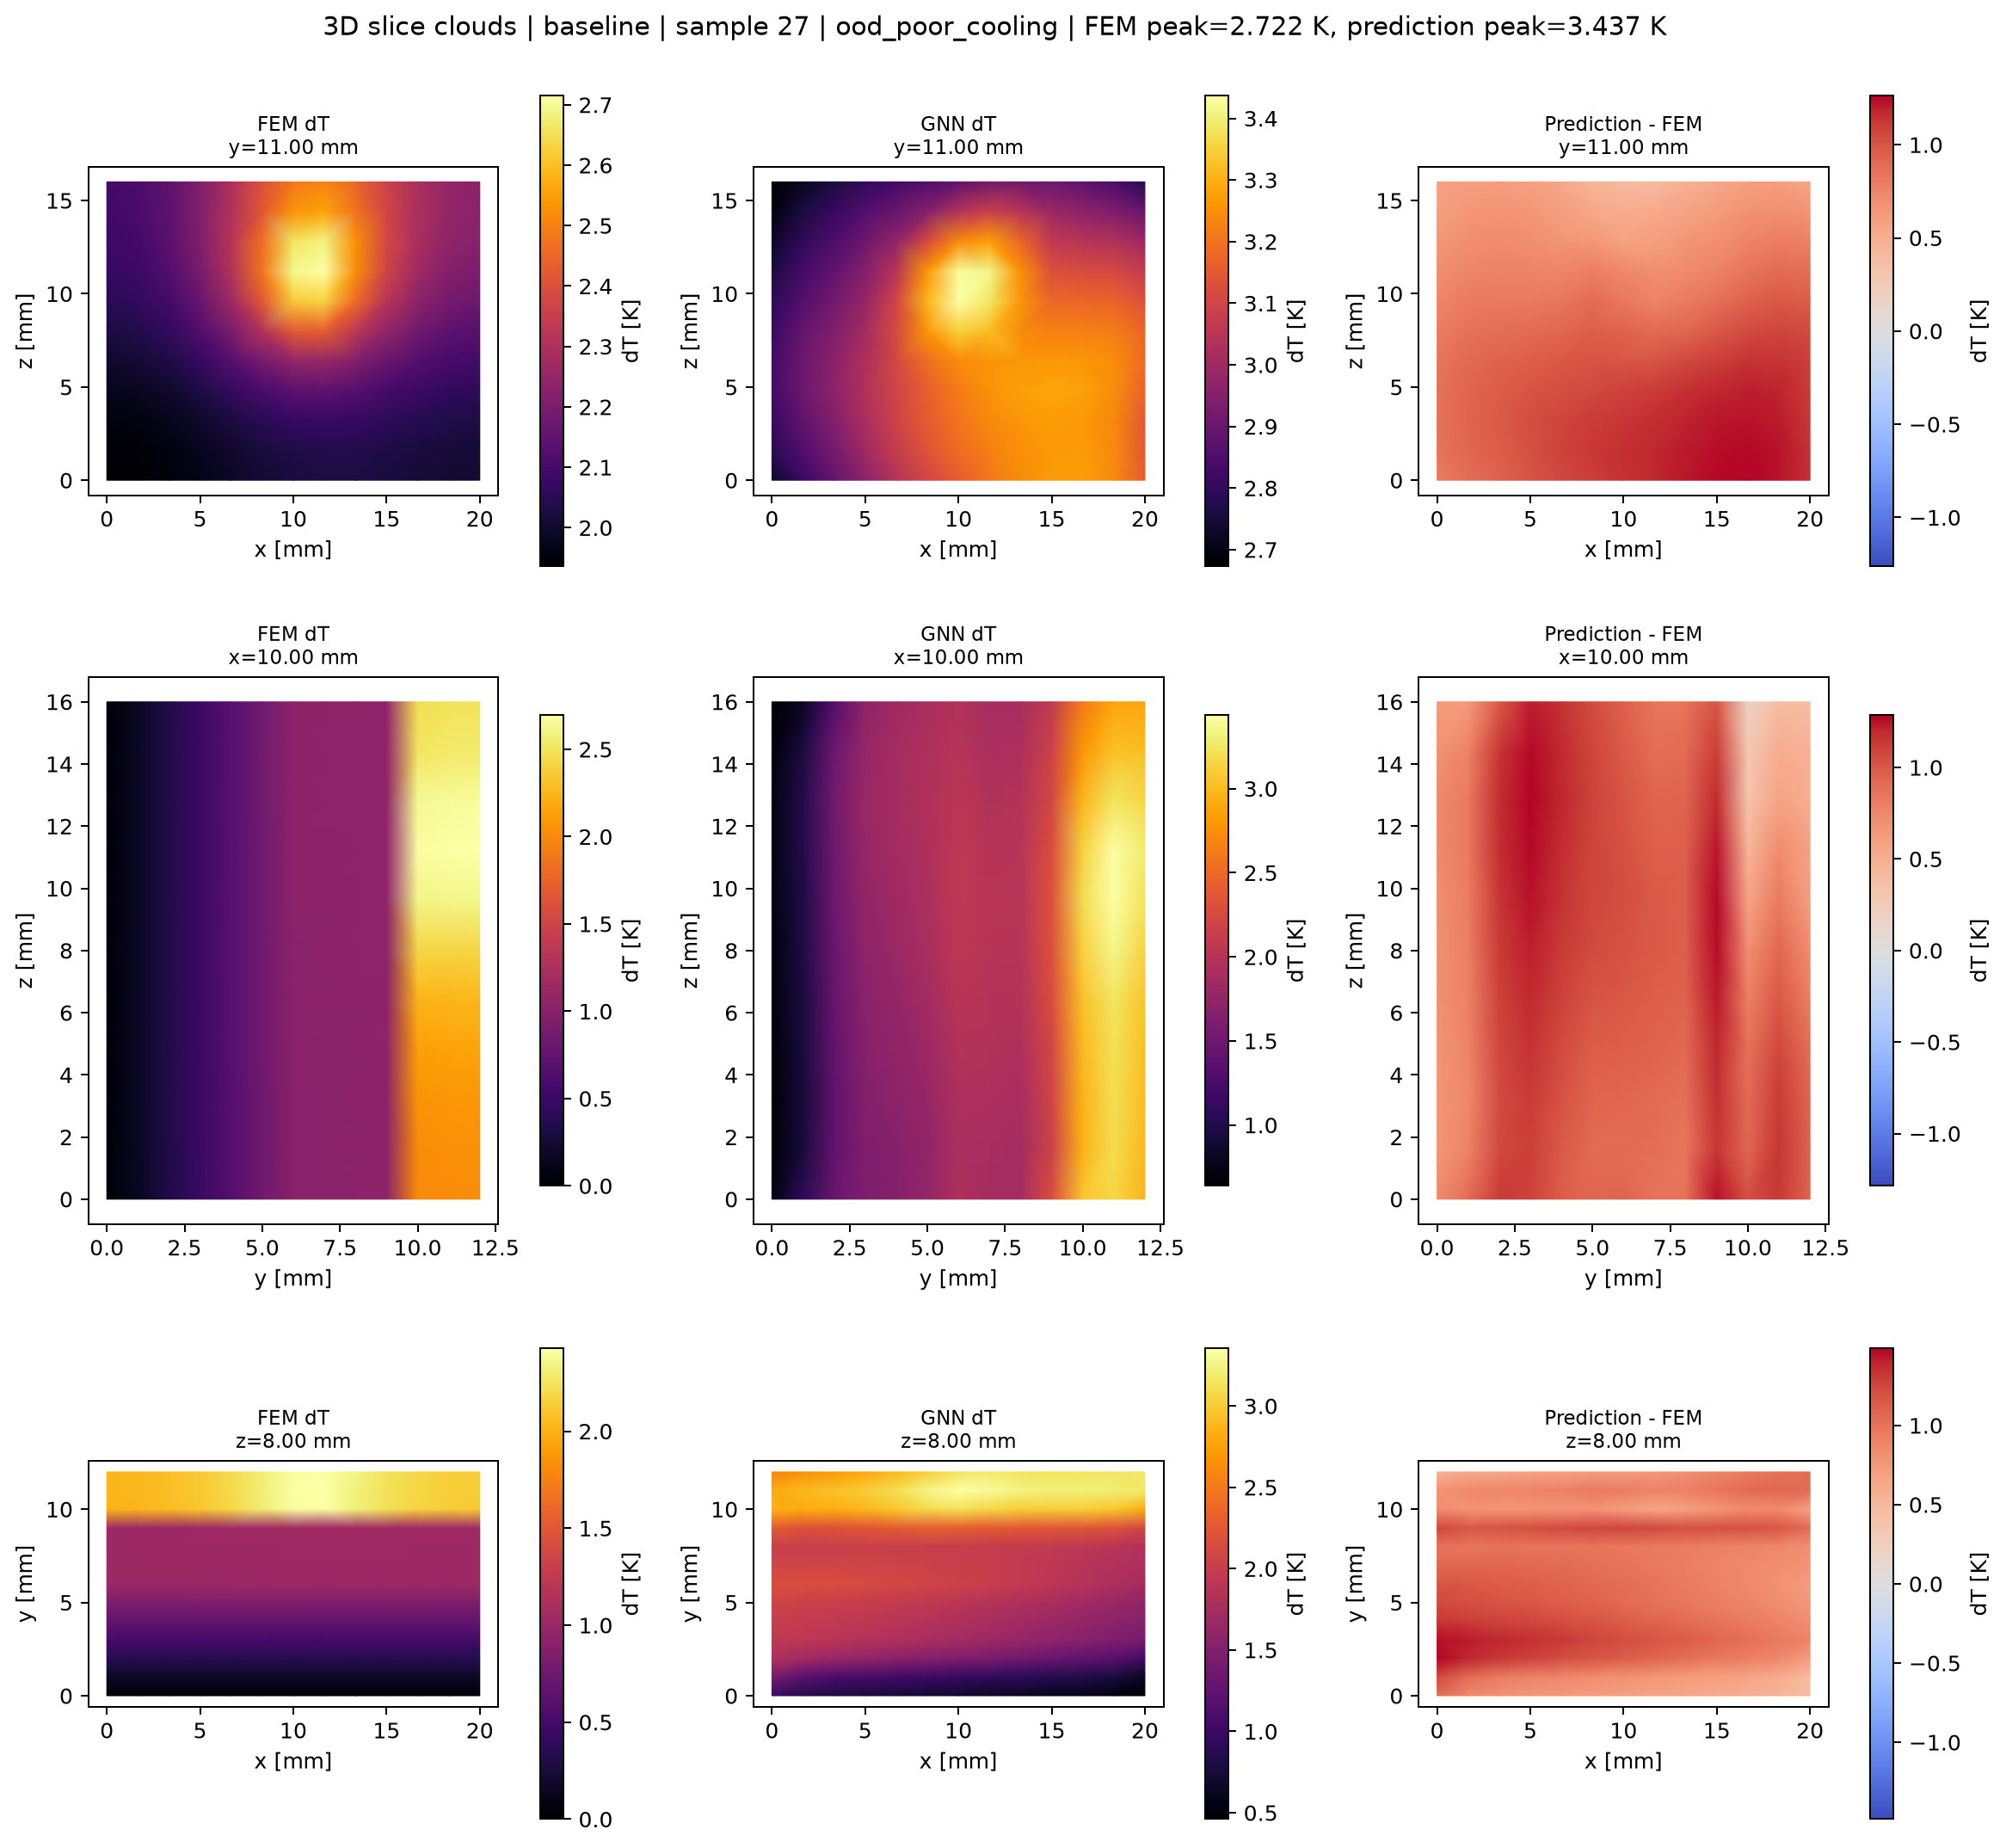
\includegraphics[width=0.98\textwidth]{slice_clouds_baseline_sample27_ood_poor_cooling.png}
  \caption{三维 GraphSAGE：差对流 OOD 样本 \#27。FEM 峰值 2.722 K，预测峰值 3.437 K。模型在三个切面均有大范围整体高估，直观对应 0.5283 K 的该工况 MAE。}
  \label{fig:3d-ood}
\end{figure}

\begin{figure}[H]
  \centering
  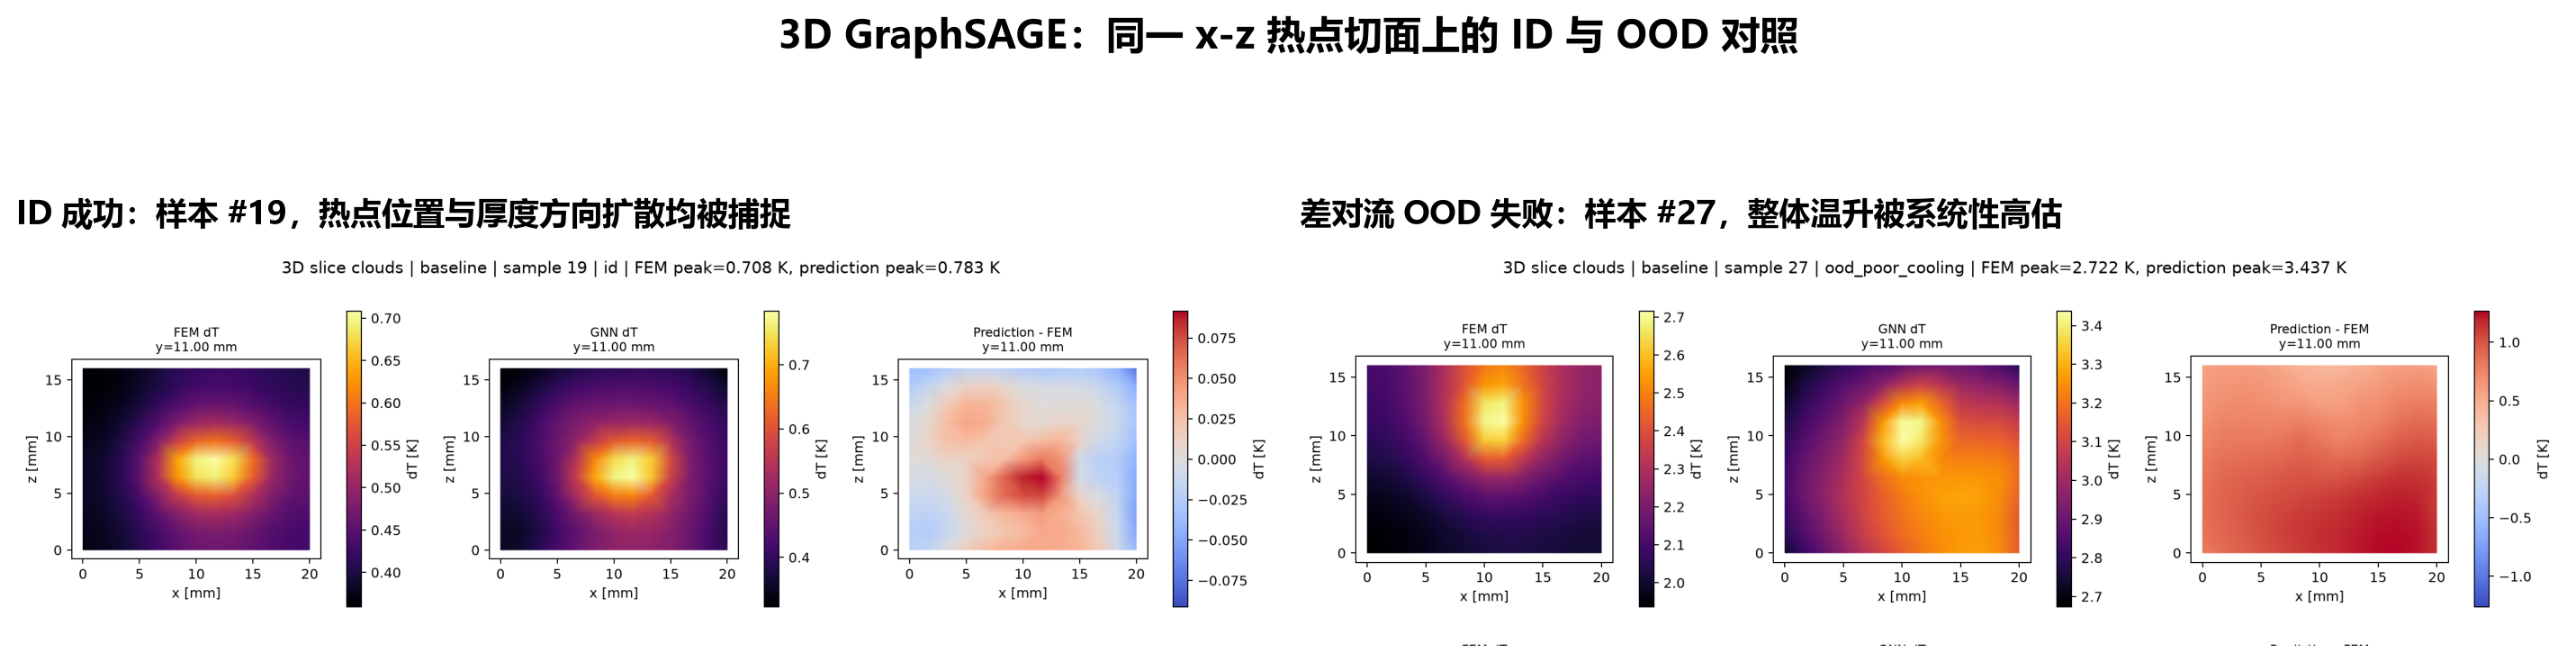
\includegraphics[width=0.98\textwidth]{id_vs_ood_success_failure.png}
  \caption{ID 成功与差对流 OOD 失败的直接对照，仅展示同一 $x$--$z$ 热点切面以保证可读性。左侧热点空间位置和厚度方向扩散基本一致；右侧预测温升在面内被整体高估。完整三切面云图见图~\ref{fig:3d-id} 和图~\ref{fig:3d-ood}。}
  \label{fig:id-ood-contrast}
\end{figure}

\subsection{二维与三维的审慎对比}
\begin{table}[H]
\centering
\caption{GraphSAGE 的二维与三维对比}
\label{tab:2d-3d}
\begin{tabular}{lcc}
\toprule
指标 & 2D & 3D \\
\midrule
节点 / 有向边 & 2,257 / 13,152 & 1,859 / 22,532 \\
参数量 & 104,321 & 19,713 \\
MAE & 0.1035 K & \textbf{0.0835 K} \\
峰值误差 & 0.3431 K & \textbf{0.1206 K} \\
加权 OOD MAE & 0.2490 K & \textbf{0.1866 K} \\
平均 FEM 时间 & 8.50 ms & 112.25 ms \\
评估 RSS & 520.09 MiB & 600.84 MiB \\
\bottomrule
\end{tabular}
\end{table}

三维在当前数据上具有更低的场、峰值和 OOD 误差，但这不能简单解释为“维数提升必然更好”：二维和三维的网络宽度、层数、物理难度和速度记录不同。稳健结论是：三维提供了真实横向扩散表征，代价是更多边和明显更高的 FEM 数据生成成本。

% =========================================================
\section{开源方案、外部参考与许可边界}
% =========================================================

\begin{table}[H]
\centering
\caption{本项目采用或审查的开源方案}
\label{tab:opensource}
\begin{tabularx}{\textwidth}{lYY}
\toprule
资源 & 在本项目中的作用 & 使用边界 \\
\midrule
scikit-fem \cite{skfem} & 实际三角形/四面体 FEM 组装和稀疏求解 & 直接依赖；FEM 标签由实际求解得到 \\
PyTorch 与 PyG \cite{pytorch,pyg} & 张量训练、图数据对象和图卷积 & 直接依赖；所有权重从零训练 \\
GraphSAGE \cite{graphsage} & 归纳图神经网络基线理论 & 本项目本地构建模型，不使用外部权重 \\
MeshGraphNets \cite{mgn} & Encode--Process--Decode 架构参考 & 本地独立实现；其公开流体/结构权重不用于热任务 \\
MOOSE \cite{moose} & MMS 与网格收敛验证方法参考 & 仅方法参考；本项目独立执行 MMS \\
MFIT \cite{mfit} & 2.5D/3D 多芯粒 RC/DSS 与输入案例参考 & 已下载；GPL-3.0，未合并源码；其 Windows 不支持 Linux \code{.so}，故未运行数值对比 \\
Multi-topology Dataset \cite{multitopology} & 功率模块温度/功率/材料掩膜参考 & CC BY 4.0；已读取一个 HDF5 样本；二维顶表面绝对温度不与本项目三维节点温升直接算 MAE \\
\bottomrule
\end{tabularx}
\end{table}

Multi-topology 的已运行公开样本为 \code{Mask\_HB\_V3-0/141\_Pigbt450\_Pfwd200\_h6000}，包含 $256\times256$ 顶表面温度、功率、芯片实例和铜/陶瓷/底板掩膜。温度范围为 46.3787--155.626 $^\circ$C，6 个芯片峰值为 145.440--155.626 $^\circ$C，$h=6000$。这是一项外部数据格式与可视化参考，不构成同几何精度竞赛。

\begin{figure}[H]
  \centering
  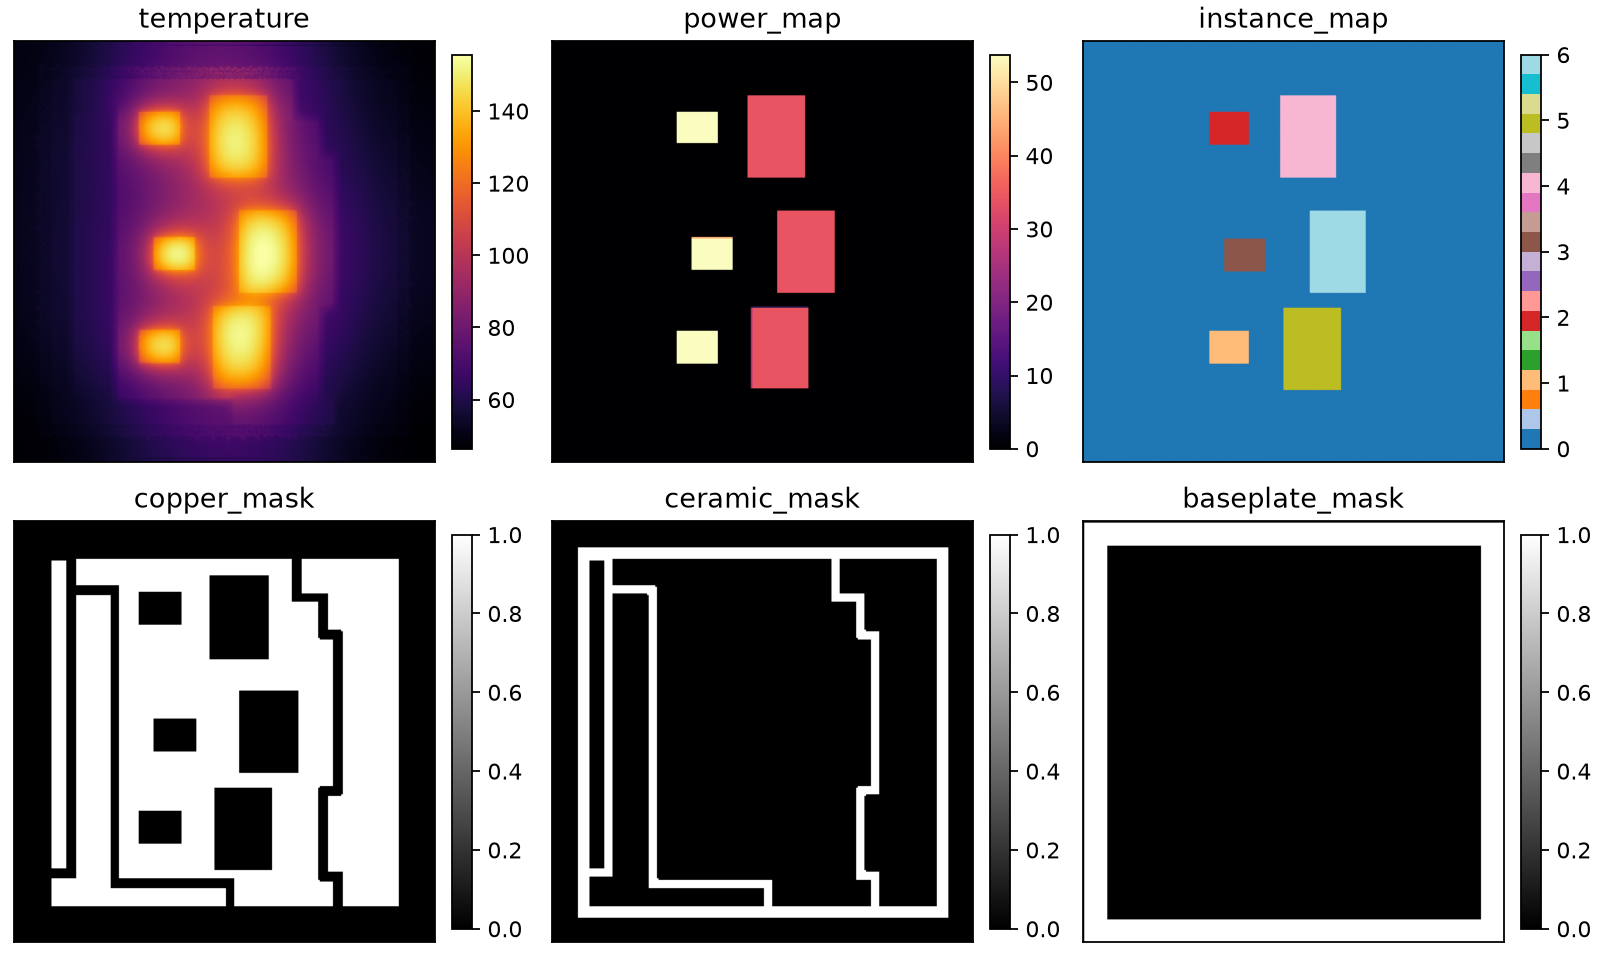
\includegraphics[width=0.95\textwidth]{reference_multi_topology_sample.png}
  \caption{Multi-topology 公共样本：温度场、功率图、芯片实例图和材料掩膜。它说明可获得的跨拓扑输入输出格式，但不是本项目三维四面体标签。}
  \label{fig:external}
\end{figure}

若与 MFIT 或其他外部求解器开展数值比较，必须统一几何、材料、功率单位、底部边界、顶面对流、绝对温度/温升定义、网格收敛准则和误差掩膜；在此之前只能进行定性或数据格式对比。

% =========================================================
\section{复现实验与产物索引}
% =========================================================

独立环境安装采用系统信任库，禁止通过关闭证书验证绕过 TLS：
\begin{lstlisting}
python -m venv .venv-3d
.\.venv-3d\Scripts\python.exe -m pip install --use-feature=truststore -r requirements.txt
\end{lstlisting}

二维数据、训练和评估：
\begin{lstlisting}
python src/generate_dataset.py --config configs/data_config.yaml --out_dir data/raw
python src/graph_dataset.py --raw_dir data/raw --out_dir data/processed
python src/train.py --model baseline --data_dir data/processed --config configs/train_config.yaml --out_dir outputs
python src/evaluate.py --data_dir data/processed --ckpt_dir outputs/checkpoints --out_dir outputs
python src/visualize.py
\end{lstlisting}

三维测试、数据、训练和云图：
\begin{lstlisting}
.\.venv-3d\Scripts\python.exe -m pytest tests/test_fem_solver_3d.py tests/test_graph_dataset_3d.py tests/test_mms_3d.py -q
.\.venv-3d\Scripts\python.exe src/generate_dataset_3d.py --config configs/data_config_3d_full.yaml --out_dir data/raw_3d_full
.\.venv-3d\Scripts\python.exe src/graph_dataset_3d.py --raw_dir data/raw_3d_full --out_dir data/processed_3d_full
.\.venv-3d\Scripts\python.exe src/train.py --model baseline --data_dir data/processed_3d_full --config configs/train_config_3d.yaml --out_dir outputs/3d
.\.venv-3d\Scripts\python.exe src/evaluate.py --data_dir data/processed_3d_full --ckpt_dir outputs/3d/checkpoints --out_dir outputs/3d --cpu_threads 4
.\.venv-3d\Scripts\python.exe src/visualize_3d.py --model baseline
\end{lstlisting}

关键产物包括：\code{outputs/metrics/*\_eval\_summary.json}、\code{outputs/3d/metrics/*\_eval\_summary.json}、\code{outputs/3d/metrics/mms\_3d\_convergence.json}、\code{outputs/figures/} 和 \code{outputs/3d/figures/}。任何改变网格、随机种子、硬件、线程、拆分或超参数的运行应写入新的输出目录，避免覆盖本基线。

% =========================================================
\section{需补充的代码与实验管线}
% =========================================================

本节列出的是\textbf{研究验证待办}，服务于证明或证伪具体假设；不是面向客户部署、批量交付或 SLA 的工程管线。工作量按一名熟悉本项目的研究者估计，不含等待计算资源的排队时间。所有新实验应保留配置、随机种子、版本与原始 JSON/CSV，且不得覆盖本报告的冻结基线。

\begin{table}[H]
\centering
\small
\caption{优先补充的代码与实验管线}
\label{tab:research-backlog}
\begin{tabularx}{\textwidth}{p{0.8cm}p{2.05cm}YYp{1.25cm}}
\toprule
优先级 & 目的（证明什么能力） & 具体做什么 & 预期产出 & 工作量 \\
\midrule
P0 & 定位最坏 OOD，而非只报平均数 & 按场 MAE/峰值排序；按四种工况导出最坏 $k$ 个样本和云图 & \code{failure\_cases.csv}、图册、归因 & 0.5--1 人日 \\
P0 & 全流程可在容差内重现 & 固定 \code{seed=2024} 串联生成、建图、训练、评估；记录版本、线程与文件哈希 & 一条命令、\code{reproducibility\_manifest.json}、核对表 & 0.5--1 人日 \\
P1 & 量化特征、峰值损失与深度的必要性 & 全局特征置零；\code{peak\_loss\_weight=0}；层数 2/3/4；保持同一划分 & \code{ablation.csv}、柱状图、结论 & 1--2 人日 \\
P1 & 分清 FEM、建图与前向的瓶颈 & 对求解、NPZ、建图、加载、前向分段计时；扫描节点/边与 batch，记录 RSS & \code{complexity\_profile.csv/json}、堆叠/标度图 & 1 人日 \\
P2 & 保证报告数字自动可追溯 & 从评估 JSON/CSV 生成含配置指纹、ID/OOD、峰值、时间和 RSS 的结果卡 & \code{results\_card.md/png}、生成脚本 & 0.5 人日 \\
P2 & 判断外部案例是否可比 & 统一单位、几何、材料、边界、温度基准与误差掩膜；同条件后才运行 & 对齐协议、检查表、对比 CSV & 1--2 人日 \\
\bottomrule
\end{tabularx}
\end{table}

\section{图表补全与阅读路径}

本节新增的图~\ref{fig:method-pipeline}、\ref{fig:model-selection}、\ref{fig:ood-breakdown} 与 \ref{fig:id-ood-contrast} 由 \code{src/generate\_technical\_report\_figures.py} 从冻结的结果摘要和既有云图产生，不会触发 FEM 或训练；原始三切面云图和外部参考图仍由各自的可视化流程生成。它们的作用与状态如下：
\begin{itemize}[leftmargin=1.5em]
  \item \textbf{端到端原型/方法流程图（图~\ref{fig:method-pipeline}，已完成）：}交代离线四面体 FEM 监督、三维 PyG 图、GraphSAGE 主基线、MGN 边属性边界与逐节点温升输出，避免把规划能力写成当前已实现能力。
  \item \textbf{ID vs OOD 对比云图（图~\ref{fig:id-ood-contrast}，已完成）：}把成功的 ID 样本与差对流失败样本放在同一视野；完整三切面留在图~\ref{fig:3d-id}--\ref{fig:3d-ood} 以支持空间判读。
  \item \textbf{OOD 分项误差图（图~\ref{fig:ood-breakdown}，已完成）：}显示差对流是最大短板，并避免只报告平均 OOD MAE。
  \item \textbf{模型对比/选型图（图~\ref{fig:model-selection}，已完成）：}用同一数据划分的误差、速度和 RSS 说明为何当前主推 GraphSAGE；该结论不外推到尚未充分训练或参数预算不同的 MGN。
  \item \textbf{消融结果图（待 P1 消融完成）：}统一展示去全局特征、去峰值损失和 2/3/4 层深度的场/峰值/OOD 误差；在没有对应运行记录前不填入假设性柱状数值。
\end{itemize}

% =========================================================
\section{局限性与后续工作}
% =========================================================
\begin{enumerate}[leftmargin=1.5em]
  \item \textbf{物理保真度：}需增加接触热阻、各向异性、温度相关材料、真实层厚、辐射和实验或高保真 FEM 校准。
  \item \textbf{网格/几何泛化：}当前每个维度中的样本共享网格；后续应随机化层厚、热点形状和网格密度，并采用跨网格测试。
  \item \textbf{OOD：}优先增加低 $h_{top}$ 样本、显式编码散热路径，并报告最坏样本/置信区间，而非只报告平均 MAE。
  \item \textbf{MGN 优化：}仅当在相同数据拆分、参数预算和指标下超过 3D GraphSAGE，才逐步增加消息传递步数或隐藏维度。
  \item \textbf{外部基准：}先在 Linux/WSL 确认 MFIT 及 SuperLU 可复现，再进行同条件 RC--FEM--GNN 比较；外部二维数据可用于迁移或跨拓扑研究，不能替代三维体场验证。
\end{enumerate}

\section{结论}
本项目已形成保留二维流程的三维热场代理基线：真实 P1 四面体 FEM、三维 PyG 图、真实后端测试、MMS 收敛、GraphSAGE 基线、紧凑 MGN 对照和三维云图均已具备。当前最可靠的下一步不是立刻扩大 MGN，而是围绕差对流 OOD 进行物理覆盖和边界特征改进，并在统一条件下引入外部高保真参考。

% =========================================================
\begin{thebibliography}{99}
\bibitem{skfem} T. Gustafsson and G. D. McBain, ``scikit-fem: A Python package for finite element assembly,'' \emph{Journal of Open Source Software}, 5(52), 2369, 2020. \url{https://doi.org/10.21105/joss.02369}
\bibitem{pytorch} A. Paszke et al., ``PyTorch: An Imperative Style, High-Performance Deep Learning Library,'' \emph{NeurIPS}, 2019. \url{https://pytorch.org/}
\bibitem{pyg} M. Fey and J. E. Lenssen, ``Fast Graph Representation Learning with PyTorch Geometric,'' 2019. \url{https://arxiv.org/abs/1903.02428}
\bibitem{graphsage} W. L. Hamilton, R. Ying and J. Leskovec, ``Inductive Representation Learning on Large Graphs,'' \emph{NeurIPS}, 2017. \url{https://proceedings.neurips.cc/paper/2017/hash/5dd9db5e033da9c6fb5ba83c7a7ebea9-Abstract.html}
\bibitem{mgn} T. Pfaff, M. Fortunato, A. Sanchez-Gonzalez and P. Battaglia, ``Learning Mesh-Based Simulation with Graph Networks,'' \emph{ICLR}, 2021. \url{https://openreview.net/pdf?id=roNqYL0_XP}
\bibitem{moose} MOOSE Framework, ``Heat Conduction Verification Tutorial.'' \url{https://mooseframework.inl.gov/releases/moose/2022-06-10/getting_started/examples_and_tutorials/tutorial03_verification/index.html}
\bibitem{mfit} A. Kanani et al., ``MFIT: Multi-Fidelity Thermal Modeling for 2.5D and 3D Multi-Chiplet Architectures.'' \url{https://github.com/AlishKanani/MFIT}
\bibitem{multitopology} R. Ke, J. Tao and C. Liu, ``Multi-topology Power Module Thermal Simulation Dataset.'' \url{https://github.com/henkuailederen/Multi-topology-Dataset}
\end{thebibliography}

\end{document}
